\documentclass[
11pt, % The default document font size, options: 10pt, 11pt, 12pt
twoside, %oneside, % Two side (alternating margins) for binding by default, uncomment to switch to one side
english, % ngerman for German
onehalfspacing, % Single line spacing, alternatives: onehalfspacing or doublespacing
%draft, % Uncomment to enable draft mode (no pictures, no links, overfull hboxes indicated)
nolistspacing, % If the document is onehalfspacing or doublespacing, uncomment this to set spacing in lists to single
liststotoc, % Uncomment to add the list of figures/tables/etc to the table of contents
%toctotoc, % Uncomment to add the main table of contents to the table of contents
parskip, % Uncomment to add space between paragraphs
%nohyperref, % Uncomment to not load the hyperref package
headsepline, % Uncomment to get a line under the header
%chapterinoneline, % Uncomment to place the chapter title next to the number on one line
%consistentlayout, % Uncomment to change the layout of the declaration, abstract and acknowledgements pages to match the default layout
]{MastersDoctoralThesis} % The class file specifying the document structure
\usepackage[utf8]{inputenc}
\usepackage[T1]{fontenc}
\usepackage{mathpazo}
\usepackage{graphicx}
\usepackage{amsmath}
\usepackage{array}
\usepackage{booktabs}
\usepackage{fullpage}
\usepackage{graphicx}
\usepackage{threeparttable}
\usepackage{wasysym}
\usepackage[ddmmyyyy]{datetime}
\usepackage{listings}
\usepackage{acronym}
\usepackage{enumerate}
\usepackage{enumitem}
\graphicspath{{images/}}
\usepackage{xcolor}
\newcommand\furtherwork[1]{\textcolor{red}{#1}}

\usepackage{hyperref}
\usepackage[autostyle=true]{csquotes}

\DeclareUnicodeCharacter{2217}{*}
\usepackage[british]{babel}
\usepackage[
backend=biber,
style=ieee,
sorting=none,
urldate=long,
doi=false,
isbn=false
]{biblatex}
 
\definecolor{codegreen}{rgb}{0,0.6,0}
\definecolor{codegray}{rgb}{0.5,0.5,0.5}
\definecolor{codepurple}{rgb}{0.58,0,0.82}
\definecolor{backcolour}{rgb}{0.95,0.95,0.92}
 
\lstdefinestyle{mystyle}{
    backgroundcolor=\color{backcolour},   
    commentstyle=\color{codegreen},
    keywordstyle=\color{magenta},
    numberstyle=\tiny\color{codegray},
    stringstyle=\color{codepurple},
    basicstyle=\ttfamily\footnotesize,
    breakatwhitespace=false,         
    breaklines=true,                 
    captionpos=b,                    
    keepspaces=true,                 
    numbers=left,                    
    numbersep=5pt,                  
    showspaces=false,                
    showstringspaces=false,
    showtabs=false,                  
    tabsize=2
}
 
\lstset{style=mystyle} 
 
\addbibresource{bibs/project.bib}
\DeclareSourcemap{ % Used when .bib/Bibliography is compiled, not when document is
    \maps{
        \map{ % Replaces '{\_}', '{_}' or '\_' with just '_'
            \step[fieldsource=url,
                  match=\regexp{\{\\\_\}|\{\_\}|\\\_},
                  replace=\regexp{\_}]
        }
        \map{ % Replaces '{'$\sim$'}', '$\sim$' or '{~}' with just '~'
            \step[fieldsource=url,
                  match=\regexp{\{\$\\sim\$\}|\{\~\}|\$\\sim\$},
                  replace=\regexp{\~}]
        }
        \map{ % Replaces '{\$}'
            \step[fieldsource=url,
                  match=\regexp{\{\\\x{26}\}},
                  replace=\regexp{\x{26}}]
        }
    }
}

\geometry{
	paper=a4paper, % Change to letterpaper for US letter
	inner=2.0cm, % Inner margin
	outer=2.0cm, % Outer margin
	bindingoffset=.5cm, % Binding offset
	top=1.5cm, % Top margin
	bottom=1.5cm, % Bottom margin
	%showframe % Uncomment to show how the type block is set on the page
}

\thesistitle{Towards Auditing of Control Flow Integrity}
\author{Luke \textsc{Atherton}}

\AtBeginDocument{
\hypersetup{pdftitle=\ttitle} % Set the PDF's title to your title
\hypersetup{pdfauthor=\authorname} % Set the PDF's author to your name
}

\newif\iflitreview
%\litreviewtrue 
\litreviewfalse

\newif\ifnotesincluded
\notesincludedtrue 
%\notesincludedfalse 

\begin{document}

\frontmatter
\pagestyle{plain}

\begin{titlepage}
    \begin{center}      
		\LARGE
		Student Number: 100905113\\
		Luke Atherton		
		        
        \vspace*{1cm}
        
        \Huge
        \textbf{Towards Auditing of Control-Flow Integrity}
 
        \vspace{0.5cm}
        \LARGE
        Supervisor: Konstantinos Markantonakis
 
        \vspace{1cm}
 
        \vfill
        
 		\large
        Submitted as part of the requirements for the award of the\\
        MSc in Information Security\\
        at Royal Holloway, University of London.
 
        
\includegraphics[width=0.4\textwidth]{royalholloway.jpg}
        
        \Large
        
        \date{\today}
        
 
    \end{center}
    \normalsize

\noindent
I declare that this assignment is all my own work and that I have acknowledged all quotations from published or unpublished work of other people.  I also declare that I have read the statements on plagiarism in Section 1 of the Regulations Governing Examination and Assessment Offences, and in accordance with these regulations I submit this project report as my own work.

\noindent
Signature:
			
\noindent
Date:
\end{titlepage}

\iflitreview

\else

\fi
\ifnotesincluded

\chapter*{Acknowledgements}
Thanks everyone! Elisabeth

\fi

\tableofcontents
\lstlistoflistings
\listoffigures
\listoftables

\begin{abbreviations}{ll} % Include a list of abbreviations (a table of two columns)
\textbf{BBL} & \textbf{B}asic \textbf{B}\textbf{L}ock\\
\textbf{SS} & \textbf{S}hadow \textbf{S}tack\\
\textbf{CFG} & \textbf{C}ontrol-\textbf{F}low \textbf{G}raph\\
\textbf{CFI} & \textbf{C}ontrol-\textbf{F}low \textbf{I}ntegrity\\
\textbf{PC} & \textbf{P}rogram \textbf{C}ounter\\
\textbf{RISC} & \textbf{R}educed \textbf{I}nstruction \textbf{S}et \textbf{C}omputer\\
\textbf{ASLR} & \textbf{A}ddress \textbf{S}pace \textbf{L}ayout \textbf{R}andomisation\\
\textbf{MAC} & \textbf{M}essage \textbf{A}uthentication \textbf{C}ode\\
\textbf{PUF} & \textbf{P}hysical \textbf{U}nclonable \textbf{F}unction\\
\textbf{RAM} & \textbf{R}andom \textbf{A}ccess \textbf{M}emory\\
\textbf{NVM} & \textbf{N}on-\textbf{V}olatile \textbf{M}emory\\
\textbf{CPU} & \textbf{C}entral \textbf{P}rocessing \textbf{U}nit\\
\textbf{ROP} & \textbf{R}eturn-\textbf{O}riented \textbf{P}rogramming\\
\textbf{ICS} & \textbf{I}ndustrial \textbf{C}ontrol \textbf{S}ystem\\
\textbf{ECB} & \textbf{E}lectronic \textbf{C}ode \textbf{B}ook\\
\textbf{OS} & \textbf{O}perating \textbf{S}ystem\\
\textbf{RTOS} & \textbf{R}eal-\textbf{T}ime \textbf{O}perating \textbf{S}ystem\\
\textbf{IoT} & \textbf{I}nternet \textbf{o}f \textbf{T}hings\\
\textbf{ROM} & \textbf{R}ead-\textbf{O}nly \textbf{M}emory\\
\textbf{FPGA} & \textbf{F}ield \textbf{P}rogrammable \textbf{G}ate \textbf{A}rray\\
\textbf{SCS} & \textbf{S}hadow \textbf{C}all \textbf{S}tack (same as Shadow Stack)\\
\textbf{ISA} & \textbf{I}nstruction \textbf{S}et \textbf{A}rchitecture\\
\textbf{IP} & \textbf{I}ntellectual \textbf{P}roperty\\
\textbf{TPM} & \textbf{T}rusted \textbf{P}latform \textbf{M}odule\\
\textbf{TEE} & \textbf{T}rusted \textbf{E}xecution \textbf{E}nvironment\\
\textbf{GPA} & \textbf{G}raphics\textbf{P}rocessing \textbf{U}nit\\
\textbf{SoC} & \textbf{S}ystem \textbf{o}n \textbf{C}hip\\
\textbf{SRAM} & \textbf{S}tatic \textbf{RAM}\\
\textbf{DoS} & \textbf{D}enial \textbf{o}f \textbf{S}ervice\\
\textbf{DEP} & \textbf{D}ata \textbf{E}xecution \textbf{P}revention\\
\textbf{JOP} & \textbf{J}ump-\textbf{O}riented \textbf{P}rogramming\\
\textbf{MCU} & \textbf{M}icro \textbf{C}ontroller \textbf{U}nit\\
\textbf{ASIC} & \textbf{A}pplication-\textbf{S}pecific \textbf{I}ntegrated \textbf{C}ircuit\\
\textbf{CISC} & \textbf{C}omplex \textbf{I}nstruction-\textbf{S}et \textbf{C}omputer\\
\end{abbreviations}


\chapter*{Executive Summary}
\addchaptertocentry{Executive Summary}
Control-flow integrity is a fundamental problem in computer security. Many attacks on software can be represented as a violation of a control-flow graph - the graphical representation of the legitimate control flow of an application. Attacks on hardware can be used to force the skipping of instructions, making the targeted application take a path which does not belong to the legitimate control-flow graph. Software-based attacks such as buffer overflows may target return addresses stored on an application's stack in order to divert its control-flow such that it does not follow the legitimate control-flow graph. Defences for attacks on control-flow attacks exist on general purpose computers, however due to resource constraints, embedded systems are less well catered for in terms of control-flow integrity. Producing an audit trail of control-flow enables a verifier to gain assurances that applications have been executed in such a way that they legitimately followed their pre-defined control-flow graph.

In order to address the problem stated above, this project surveys existing solutions in the area of control-flow integrity. Initially it undertakes a high-level review of secure software execution, associated subjects and the common properties for embedded systems. Following this it sets out an established criteria for the assessment of solutions providing static attestation of memory space and control-flow integrity protection and attestation. Using this criteria these solutions are analysed and compared. The solutions presented consist of hardware-based solutions, where additional hardware components or modifications are required, and software-based solutions, where objectives are achieved using only software and existing Commercial off-the-shelf (COTS) hardware.

In its concluding chapters, the project builds upon the principles and methodologies identified during the analysis and comparison phase to propose a solution that enables auditing of control-flow within embedded systems. Using a combination of static attestation and dynamic monitoring, the proposed solution aims to provide the building blocks for a software-based design anchored on the security features provided by ARM TrustZone (recently added to ARM Cortex-M processor cores, which are at the heart of many embedded systems). Finally, it is recommended that the proposed solution is implemented in a hardware-based solution, where any overhead introduced as a result of the functionality can be reduced by introducing dedicated hardware.


\iflitreview

\chapter{Literature Review}
This chapter analyses and summarises contributing and related academic work applicable to this project. In the first section we will discuss works which describe the problems to be addressed and existing solutions to said problems, this section also includes a subsection on FPGA security which makes for useful reading as many embedded systems are FPGA-based. The second section contains a brief review of other physical attacks not addressed in the first section. We then undertake a deeper analysis of a handful of existing solutions, some of which directly address binding of software and hardware and some of which focus on the related subject of secure software execution. The fourth section provides a brief introduction into some of the founding principles used in many of the solutions already described and should be useful knowledge to have with respect to this project.

\section{Subject-matter Surveys}\label{subjectMatterSurveys}

Many surveys on solutions which increase security for firmware/software in embedded systems have been completed. One such survey \cite{Shepherd2016} focusses on existing mature solutions, while others \cite{Bryant2004}, \cite{Collberg2002} and \cite{Theissing2013} provide a look at broader principles. All of these surveys also paint a picture of the attacks and threats which embedded systems face. Other surveys exist on the technologies described in this project, one such survey is \cite{Drimer2008} which focuses on FPGA security.

These subject-matter surveys will be discussed in \ref{solutionSurveys} and \ref{faultInjectionDefenceSurveys} and a deeper analysis of some of the solutions presented will be discussed in \ref{bindingSolutions}, \ref{secureExecutionSolutions} and \ref{staticAttestationSolutions}.


\subsection{Surveys on Existing Solutions for IP Protection and Secure Execution}\label{solutionSurveys}

A survey in to technologies designed to ascertain trust for embedded systems is provided in \cite{Shepherd2016}. In this, the authors compare various technologies, some of which are mature and some in their infancy. Studied solutions include: Trusted Platform Module (TPM), Secure Elements(SE), hypervisors and virtualisation (e.g. Java Card and Intel's Trusted eXecution technology), Trusted Execution Environments (TEEs), Host Card Emulation (HCE) and Encryption Execution Environments (E3 - which has also been directly discussed in \cite{Lee2016}). The paper's authors set out a series of criteria which solutions are tested against, including such criteria as ``Centralised Control', where the trust technology is under the control of the issuer or the maintainer, and ``Remote Attestation'' where the trust technology provides assurance to remote verifiers that the system is running as expected. The paper goes on to describe each technology in a small amount of detail and populates a matrix of technologies vs. criteria. 

In a survey of anti-tamper technologies \cite{Bryant2004}, a series of \textit{cracking} threats and software and hardware protection mechanisms are described, many of which apply to embedded systems. Such threats include: 
\begin{itemize}
	\item Reverse engineering, achieved through a variety of methods including gaining an understanding	of software or simply \textit{code lifting} where sections of code are re-used without understanding of their functionality;
	\item Violating code integrity, where code is injected into a running program to make it carry out illegal actions outside of the desired control-flow of the program.
\end{itemize} 
Hardware solutions described include: using a trusted processor used to secure the boot of the system, using hardware to decrypt encrypted software from the hard-drive and RAM, using a hardware \textit{token} which is required to be present for the software to run.

The advantages of using hardware solutions include: using a complex CPU which is difficult to defeat while not redirecting resource from the processor used for standard operation, it is more costly to repeat attacks on hardware than it is for software (physical access is required each time) and secure hardware can also control which peripherals can be connected to the system and which software (signatures) can be allowed to run. There are some disadvantages of using hardware solutions which need to be considered, including:
\begin{itemize}
	\item Secure data traversing the secure to non-secure boundary needs to be encrypted (which creates an additional overhead for the main processor)
	\item Hardware solutions tend to be inflexible and less secure than commonly assumed
	\item Additional components can add to the cost of manufacture, which is a high priority for embedded systems design.
\end{itemize}
Software solutions described include:
\begin{itemize}
	\item Encryption wrappers, where all or just the critical portions of software are stored in a ciphertext form and dynamically decrypted. The value of this is that the attacker will not see all of the source program at the same time, however they can piece it together through snapshots or simply learn the encryption key/s. This paper does not cite any references for the subject of encryption wrappers, which could suggest that encryption wrappers are not widely researched;
	\item Code obfuscation, where the look of the code is adjusted to make it not easily readable or understandable by the attacker but performs in the same manner;
	\item Software watermarking and fingerprinting, which can be used for proof of ownership or authorship and for finding the source of leak of the software;
	\item Guarding, which is the act of adding code purely to perform anti-tamper functionality. An example of guarding is comparing checksums of running code to expected value and performing certain actions if they do not match. It is recommended that guarding is implemented automatically rather than manually as providing sufficient coverage is a complex task. It is also noted that a guard should not react immediately so as to not reveal the point in the code which triggered it.
\end{itemize}
The paper also describes a series of steps to take when using anti-tamper technology as put forward by the ``Defence Acquisition Guidebook'' created by the Defence Acquisition University \cite{DAU2011}.

A similar survey \cite{Collberg2002} covers three types of attacks: reverse engineering, software piracy and tampering, which it describes as ``malicious host attacks''. To defend against such attacks the paper states three corresponding defences: code obfuscation (as well as anti-disassembly and anti-debugging measures), watermarking and tamper-proofing. The authors note that they could not find a wealth of information on tamper-proofing at the time of writing (2002) but they do draw an interesting parallel with the anti-tamper mechanisms used in computer viruses.  

\subsection{Defence against fault injection}\label{faultInjectionDefenceSurveys}

A series of high-coverage tests for security protections against fault injection attacks were run and described in \cite{Theissing2013}. It describes 17 different countermeasures, including: countermeasures protecting the data layer, combinations of data protection methods, countermeasures protecting control flow layer, combinations of control flow protection methods and combinations of data and control flow protection. To test these methods the authors produced a high number of simulated fault injections on a simulator of an ARM-Cortex-M3 processor running a benchmark application representing a bank card.

The experiments found that a combination of redundant condition checks (such as data duplication) and source and destination IDs reached the best coverage with moderate performance overhead. They also found that simple ID-based inter-block control checking were able to outperform more sophisticated (and complex) methods such as Control-Flow Checking by Software Signatures (CFCSS) as seen in \cite{Werner2016} and Assertions for Control-Flow Checking (ACFC) seen in \cite{Goloubeva2003}.

\subsection{FPGA Security}

An excellent high-coverage survey on FPGA security is provided in \cite{Drimer2008}. Its contents include the background of FPGAs, attacks associated with FPGAs, defences for protecting FPGA implementations (existing at the time and ongoing research) and many more. 

\section{Attacks}

The following are some examples of analysis of threats, all of which are aimed towards disrupting the flow of software, the likes of which are the focus of secure software execution solutions. 

Attacks which can be used to break instruction-level countermeasures are described in \cite{Yuce2016a}. This paper discusses various attack countermeasures and how these are circumvented. The only countermeasures addressed in this paper are algorithm-level and instruction-level (both of which are mostly redundancy-based). This paper suggests that a purely software-based countermeasure could be a futile defence.

Findings that physical faults can be injected in a non-random manner and in a low cost environment are presented in \cite{Kelly2017}. This contradicts assumptions made in many of the examined solutions that physical attacks are too costly. It finds that instruction-skipping attacks create a vulnerability to skipped-instruction errors (which, it could be argued, drives the motivation behind control-flow monitoring right down to the intra-block level).

Further details on side-channel attacks, as well as a brief description of the security concerns associated with FPGAs are provided in \cite{GebotysCatherineH2010Sied}.

\section{Solutions} \label{solutionsDescriptions}

A myriad of creative technical solutions have been put forward which address the problems already discussed. They can be placed in to one of two categories - binding hardware \ref{bindingSolutions} (\cite{Lee2016}, \cite{Schaller2014}, \cite{Gora2010} and \cite{Simpson2006}) and software or secure software execution \ref{secureExecutionSolutions} (\cite{Werner2016}, \cite{Wang2016}, \cite{Abera2016} and \cite{Arora2006}). Hybrids of the two approaches are presented in \cite{Kleber2015} and \cite{Kohnhauser2015}.

\subsection{Binding Hardware and Software}\label{bindingSolutions}

Hardware software binding is a technique where hardware and software a co-designed in such a way that software needs to be tailored to run on an individual instance of hardware. The same principle works the other way in that an individual piece of hardware will not execute software unless is it specifically tailored to it.

The first piece of work we consider is \cite{Lee2016}. The problem the paper aims to address is device counterfeiting. An example of the requirement for binding of hardware and software is for Graphics Processing Units (GPUs), where GPUs are fabricated and then tested on their operating performance and subsequently graded. Once graded, the GPUs are loaded with firmware which controls their voltage and clockspeed. The paper states that firmware aimed towards the superior graded GPUs could be installed on lesser graded devices, which would then be rebadged and sold on as superior GPUs.

The attacker described in \cite{Lee2016} is one which has several special attributes: they have physical access the device, access to the device storage where they can read and copy the entire contents of memory, they are able to use hardware which has been built to the exact specifications as the original hardware and they can ``read and copy any data which is loaded onto any of the buses which make up the embedded system''. The attacker's aim is to either create a counterfeit platform which performs and functions in the same manner as the original or to install software retrieved from the legitimate product onto different (counterfeit) hardware.

The method presented in \cite{Lee2016} uses a function applied to either the previous contents of memory or a randomly generated number to produce a mask which is applied to the program instructions residing in memory. The intention is that the CPU unmasks the contents as part of the execution process prior to actually carrying out the operation. The paper discusses the options for the mask-creating function, suggesting the use of hash-functions, PUFs, or block ciphers before finally selecting PUFs due to their intrinsic nature. The act of masking the software has been undecided in this paper, which suggests that either the software is masked prior to loading or is masked during the loading process. The paper's author describes the provisioning process in a further paper \cite{Lee2017}.

The second piece of work we consider is \cite{Schaller2014} where the goal is to ``protect against intellectual property (IP) extraction or modification on embedded devices without dedicated security mechanisms''. In this paper the attacker is aiming to extract IP (in the form of software or secrets) stored on the device. The attacker may use this information in any of the following ways: they may implement the extracted information on counterfeit devices, they may modify the software or data to remove licensing restrictions or unlock premium features, they may downgrade to earlier firmware versions  in order exploit previous vulnerabilities, they may wish to alter firmware to capture valuable data such as password, change output data such as readings on smart meters or reveal secrets such as cryptographic keys.

In \cite{Schaller2014} the attacker is assumed to have physical access to the device, can read the contents of external memory and can inspect and modify on-chip memory values. The assumed limitations placed on the attacker by the paper are that the attacker cannot change the code of the boot-loader as it is stored in a masked read-only memory (ROM), they cannot replace the ROM chip with one with a boot-loader under the attacker's control (as the ROM chip would be heavily integrated on a system-on-a-chip (SoC) so would require skill levels outside of those expected of the attacker) and finally the attacker cannot read the start-up values of the on-chip SRAM during start-up which are protected by the boot-loader and are erased once read by the boot-loader.

The method described in \cite{Schaller2014} heavily utilises PUFs created using the SRAM start-up values to derive a key used to decrypt the firmware. The firmware is decrypted by the boot-loader before being loaded and executed. The system was implemented on a SoC platform using a two-stage bootloader (u-boot). The paper's authors provide an extensive review of SRAM PUFs for ARM Cortex-M and Pandaboard's IMAP and includes a description of Fuzzy Extractor design used by the solution.

The third piece of work \cite{Kleber2015} has not been published in a well-established journal however the authors have been invited to present their findings in \cite{Kleber2015a}. Here the problem of injection of malicious code is also addressed, as well as prevention of code reverse-engineering. This paper uses secure execution to bind hardware to software.

The attacker identified in \cite{Kleber2015} has physical access to the processor, peripheral connections and they can read out contents of memory or registers. They are also assumed to be able to place arbitrary data into the main memory of the processor (either locally or remotely). Attacks comprising denial-of-service (DoS)achieved by, for example, injection of random invalid instructions and hardware side-channel attacks have not been addressed.

The method described has been labelled ``Secure Execution PUF-based Processor'' or SEPP. The operating principle of SEPP is the encryption of basic blocks (which have exactly one entry point and one exit point) which make up programs. The blocks are encrypted using a symmetric cipher in CTR mode with the parameters set in relation to instruction location within a block and the block's location within memory. The key used for this encryption is set by the user. SEPP utilises a ring-operator (RO) PUF to create a new key used to encrypt the user's key. The decryption module is included in the instruction fetch stage of the processor's pipeline and makes use of first-in, first-out (FIFO) buffer to store encryption pads before they are needed by the processor (therefore making use of spare time provided by instructions which take more than one processor cycle). This system also implements u-boot as a bootloader which has been modified to provide the functions of the security kernel. It appears that due to the nature of this method (the device tailoring the software to itself), it does not prevent malicious uploading of a new program to the device which it then processes.

The fourth method identified in \cite{Kohnhauser2015} has identified illegitimate reproduction as a problem that requires a solution. It also identifies modification of software to bypass the need for purchasing a license for particular features as another attack scenario. Here, the attacker has the ability to read and modify the content of external memory such as flash memory or RAM. They can also do the same with internal memory including software with hard-coded secrets and cryptographic keys. The method consists of four basic mechanisms: two check functions and two response functions. The first check function hashes the native program code and compares this to the current running code. The second check function uses a SRAM-derived PUF to measure the authenticity of the device. If these functions indicate that either the software is not in its intended state or is running on the incorrect device, the first response function adjusts the flow of the program to move in a random manner and the second response corrupts the program's execution stack. Both response functions are designed to cause a malfunction in the program. One has to question the safety of having a program jump to a random block.


The fifth method described in \cite{Gora2010} is developed to protect against IP theft or reverse engineering. This paper does not describe the attacker but makes the assumption that they will not be able to access the PUF-based key used for encryption as it is internal to the FPGA. This method uses an obfuscated secure ROM to start the boot process, checking and running the integrity kernel which decrypts and runs the software using the PUF-based key. In my opinion, the problem with this solution is the reliance on an obfuscated ROM. This is because once there is an understanding of a ROM it could be possible for malicious software to be written in a manner that is accepted by the boot program in ROM.

An honourable mention should be made for \cite{Simpson2006} which was published in 2006 and led the way in using PUFs to secure software and also clearly describes the enrolment process with defined message exchanges.

\subsection{Secure execution}\label{secureExecutionSolutions}

Secure software execution (or control-flow security/integrity) has the goal of preventing the desired results of attacks against program control flow, which aim to use physical attacks to make the execution of running programs jump to blocks which should not be running at that particular time (e.g. an administration function).

The first solution, \cite{Werner2016} raises the point that most research on fault-attacks has been aimed towards cryptographic functions which result in gaining knowledge of the secret key. This paper takes this further by considering the modification of games consoles to make them skip the function which checks the validity of loaded software. The paper focuses on securing against fault-attacks.

The method mainly utilises control-flow integrity to solve the stated problem. The basic principle behind control-flow integrity is the understanding of the basic blocks of a making up a program. The blocks will transition into one another creating control-flow. This flow can be described as the control-flow graph (CFG) and a correctly functioning program will abide by this graph. The signature of the program flow is created and compared against the expected value according to the CFG. The solution provides assistance to C programmers in that it automatically inserts signature updates, although programmers can also insert them manually for critical sections of the program. This functionality has been provided via the editing of LLVM compiler. If using assembly code the programmer must manually insert signature updates whenever branches, loops and function calls are encountered. The control flow signatures are calculated through a  recursive disassembling approach. In order to check the running  program's integrity a ``derived signature'' is calculated on the running code's path, this can then be compared to the corresponding derived signature of the intended route of the CFG. Important principles introduced in this paper (along the same lines as CFG) are generalized path signature analysis (GPSA) and continuous-signature monitoring (CSM). This paper does require modifications be made to Cortex-M3 architecture.

The second paper \cite{Wang2016} (ConFirm) states that ``given the critical role of firmware, implementation of effective security controls against firmware malicious actions is essential'', having read the various prior examples seen we can safely agree with this. 

The attacker is assumed to have the ability to inject and execute malicious code, or call existing functions not abiding by the control-flow graph. These attacks are assumed to be possible either on-line or off-line (which would require a device to reboot after uploading of a malicious firmware image) and depending on the design of the device the firmware alterations could be achieved locally or remotely.

The method employed revolves around making use of hardware performance counters (HPCs) which count various types of events. The HPCs are utilized in conjunction with a bootloader (which sets checkpoints, initialises an HPC handler and contains a database of valid HPC-based signatures). While the program is run, HPC values are checked once checkpoints are reached (checkpoints are placed at the beginning and end of each basic block, as well as one randomly inserted between). The checkpoints actually redirect the control flow to the ConFirm core module to compare the HPC value with those stored in the database containing valid values. If the check fails ConFirm will report a deviation, which could be used to run a fault sequence, such as ``rebooting the system, generating an alarm and disabling the device''.

The third paper \cite{Abera2016} approaches secure execution from a slightly different direction: remote attestation. It aims to provide remote attestation of an application's control flow path during operation. The paper excludes physical attacks and instead focusses on execution path attacks. They assume that the subject device features data execution prevention (DEP) such as read $\oplus$ write and a secure trust anchor that provides an isolated measurement engine and can generate the fresh authenticated attestation report.

The method builds a hash of the path taken from node to node which is then reported to the verifier. Loops are dealt with in a novel manner to work around the issue posed due to the infinite hash available when the number of iterations of a loop is set dynamically.

The fourth paper \cite{Arora2006} lists various attacks, ranging from buffer overflow attacks to physical attacks. Their method measures inter-procedural control flow, intra-procedural control flow and instruction stream integrity. Control flow monitoring is provided by an additional hardware element which tracks instruction addresses and compares them to known acceptable values stored in lookup tables. Instruction steam integrity monitoring utilises the lookup tables in addition to corresponding hash values of the basic clock. If a violation is discovered it is reported to the processor which should then terminate execution of the current program. Details of the violation are included in the report to the processor to enable a finer-grained view of the violation.

\section{Primitives}

\subsection{Control-flow Graphs}

The use of control flow checking for accidental program flow changes is considered in \cite{Goloubeva2003}, and explains the basic principle well. It describes basic blocks, control-flow between blocks, how these make up program graphs and finally how these graphs can be used to indicate control-flow error. The paper presents two existing error detection methods but finds faults in both so presents a novel solution addressing the previous solutions' shortcomings.

Chapter 9 of \cite{AhoAlfredV.2014C:pt} contains a wealth of information on data-flow and will provide a good basis for understanding both the essence of data(control)-flow and how compilers use them for code optimisation. This chapter should be referenced in order to gain a meaningful understanding of control-flow.


\subsection{Physical Unclonable Functions (PUFs)}\label{PUFExplaination}

A huge amount of prior research has been undertaken into PUFs and their application towards security in embedded systems. A good overview is the PhD thesis \cite{Maes2012}, which provides a thorough examination into most aspects of PUFs including the types, analysis of each type in terms of uniqueness and reproducibility and uses including entity-authentication and key generation.

Much of the literature (\cite{Lee2016}, \cite{Schaller2014}, \cite{Kleber2015}, \cite{Kohnhauser2015}, \cite{Gora2010} and \cite{Simpson2006}) already described explain the use of PUFs and their reasoning behind their choice in PUFs.

\section{Chapter Summary}

In this literature review we have seen the reasons why the security of firmware of embedded devices is an important matter which needs to be addressed. We then saw reviews of existing solutions and introductions to primitives used. After an introduction to potential physical attacks we then provided an in depth review of solutions which enabled the binding of hardware and software and solutions which provide secure software as well as attestation of code. Finally we looked at two primitives which were prominent in many of the solutions examined.


\appendix
\chapter{Appendix Title}
This is my appendix
\else

\mainmatter
\pagestyle{thesis}

\chapter{Introduction}
In this chapter we first introduce the concept of control-flow, describing how it is built up from transitions between basic blocks to form a control-flow graph and how control-flow can be violated. We then look at the types of execution branches which trigger transitions between basic blocks. We explain some important categories of hardware and software attacks which can lead to the subversion of a control-flow. Finally the problem setting for this project is described along with a list of objectives which the proposed solution will be judged against.
\section{Control Flow}
Control flow is how instructions within software applications transition from one instruction to another. Applications can be logically broken down into basic blocks (BBLs) through which the executing application traverses. The tracing of these transitions forms the control flow taken.

\subsection{Basic Blocks}
The principle of basic blocks creates a useful way of breaking down the instructions of an application into manageable chunks containing sequences of instructions. A basic block is a set of instructions which sequentially run from beginning to end. An example of this is illustrated in pseudo-code at listing~\ref{lst:basic_code}.

\begin{lstlisting}[language={[Sharp]C},caption={An example of code which can be broken down into basic blocks},label={lst:basic_code}]
void GreaterThanPlusOne(int firstNum, int secondNum)
    {
        string message;
        firstNum++;
        if (firstNum > secondNum)
        {
            message = "firstNum plus one is greater than secondNum";
        }
        if (firstNum <= secondNum)
        {
            message = "firstNum plus one less than or equal to secondNum"
        }
    }
\end{lstlisting}

The instructions from \verb|string message;| (line 3) up to and including \verb|if (firstNum > secondNum)| (line 5), \textit{basic block 1}, will execute sequentially (barring an exception being thrown). This is a basic block. The contents within the first \verb|if| (line 5) and also the second \verb|if| (line 9) parenthesis are also basic blocks, \textit{basic blocks 2 and 3} respectively.

So in the code described at listing~\ref{lst:basic_code}, the sequence of instructions can flow from the first basic block to either the second or the third. An unauthorised flow would be from basic block 2 to basic block 3 as there is no way that under normal operation both of these sequences of instructions would execute after one another.

Other examples of programming control flow statements which could form basic blocks are switch cases, loops, break statements and functions, as the these control the diversion of instruction execution depending on the current running circumstances (e.g. variable state).

\begin{figure}
  \centering
  \vspace*{0.5in}
  \includegraphics[scale=1]{cfg.png}
  \caption{The control-flow graph for code in listing~\ref{lst:basic_code}}
  \label{fig:basicCFG}
\end{figure}

\subsection{Control-flow graphs}
Control-flow graphs (CFGs) are the graphical representation of the series of valid transitions between basic blocks within an application (see figure~\ref{fig:basicCFG} for a CFG of listing~\ref{lst:basic_code}). It is conceivable that a CFG can become enormous as the size of an application grows, as the number of different valid paths along the graph will rapidly increase.
\ifnotesincluded
\furtherwork{(need to find reference for this)}
\fi. Valid control flow is where the flow which follows a CFG for a given application. Using figure \ref{fig:basicCFG} as an example for the code in listing \ref{lst:basic_code}, BBL 1 $\rightarrow$ BBL 2 and BBL 1 $\rightarrow$ BBL 3 are both valid flows, however BBL 1 $\rightarrow$ BBL 2 $\rightarrow$ BBL 3 is invalid. To create BBL 1 $\rightarrow$ BBL 2 $\rightarrow$ BBL 3 an attacker could change the value of \verb|secondNum| to one which is greater than or equal to \verb|firstNum| once the first \verb|if| statement has been passed. 

\subsection{Types of branches}
In order to understand control-flow it is important to understand the difference between the various branch types: direct, indirect, unintended and function returns.

\subsubsection{Direct}
A direct branch is one where the next instruction address is hard coded with the \verb|jump| instruction. This means the execution will flow to a pre-defined location.

A direct branch can be violated by hardware attacks such as glitching, which forces the skipping of instructions, or memory attacks, whereby the destination address is swapped for another, causing the execution to flow along an unintended path.

Attacks on direct branches can often be overlooked by control-flow integrity (CFI) protection mechanisms as the requirements of needing direct access to memory or performing glitching attacks often lie outside of the scope of these protections, as they view attacks on indirect branches and function returns as larger threats.

\subsubsection{Indirect}
An indirect branch is one where the next instruction address is set at run-time, either through registers, or pointers pointing to addresses in memory containing the \verb|jump| destination. This could be the result of a compiled \verb|switch|-\verb|case| statement or dynamic libraries (e.g. reflection). In the case of the \verb|switch|-\verb|case| statement it might not appear as indirect in the source code, however when compiled has the possibility of indirectness. Indirect branches are usually targets of buffer overflows.

\subsubsection{Unintended}
De Clerq \cite{DeClercq2017} describes an unintended branch as one which arises due to variable length instruction encoding in architectures. An attacker transfers control flow to the middle of an instruction. A high percentage (80\%) of gadgets exploit this, according to Kayaalp \cite{Kayaalp2014}. For more information see section 4.2 of Kayaalp's work \cite{Kayaalp2014} which describes unintended branches in detail. The threat of unintended branches is currently not such a problem in embedded systems as they tend to use fixed length instruction sets (such as RISC). However ARMv8, for example, has two sets of encoding which can be switched between, and as embedded systems' capabilities converge with those of general purpose computers we may see the introduction of variable length instruction encoding in the near future.

\subsubsection{Function Return}
A function returning to its caller is a branch in itself. When a function returns to its calling section of code the return address is retrieved from the stack and inserted in to the program counter (\verb|pc|). This presents a problem as the return address is not hard coded and according to a CFG, a function could legally return to any of the locations in code which call that function. Tracking the entire path taken along the CFG allows the checking of calling location, making sure the function has returned to the correct caller.

If the stack is attacked the return address can be re-written to point to existing code, or instructions placed in data (this is usually protected for by read $\oplus$ write). This is a well-explored area in computer security with various existing solutions including stack canaries, NX bit and Address Space Layout Randomisation (ASLR).

\ifnotesincluded

\subsubsection{Break statements}

\furtherwork{Should these be included?}

\fi

\subsection{Loops}
Loops are problematic in terms of CFGs. Modelling a loop which could run indefinitely is simply not feasible if full coverage is to be achieved. Various methods have been used to approach this, with some \cite{Abadi2005} simply compacting loops (this presents issues where an attacker can continually run a loop until they reach the desired outcome, such as performing an exhaustive search on passwords) while others \cite{Dessouky2017} track loop metadata such as iteration count for each unique path taken through a loop.
\UseRawInputEncoding
\section{Attacks on Hardware} \label{hardwareAttacks}

Attacks on hardware are amongst the hardest attacks to mitigate against, as having direct access to memory or even cache memory can enable an attacker to bypass many protections (for example software-based protections). Hardware attacks can be used to capture the leaking of cryptographic keys, which presents a problem, particularly for attestation where a typical attestation report is signed using a signing key or when a symmetric key is used for encrypting or applying a MAC to the attestation report. The basis for this section stems from \cite{MayesKeithE2008SCTS} where attacks on hardware which are applicable to embedded systems are well explored.

\subsection{Invasive Attacks}
An invasive attack occurs when a microprocessor is removed and attacked directly through physical methods. In theory any microprocessor can be attacked in this way however it does require expensive equipment and a large investment in time.

One example of an invasive attack is probing bus lines between blocks on a chip (with a hole being made in a chip's passivation layer). Here, secret information is derived by observing information sent from one block to another. An extreme example of an invasive attack is using a focused ion beam to destroy or create tracks on the chip's surface. This could be used to reconnect disconnected fuses (this is a threat to the use of PUFs (see \ref{PUFExplaination} for more details) where fuses are used to deactivate PUF derivation circuits). Fuses can also be used to turn off test modes which are used to read\slash write to memory addresses during manufacture. Modern solutions avoid this vulnerability by removing test circuits from the chip when it is cut from the die during the manufacturing process \cite{Anderson1996},\cite{Kommerling1999}.

\subsection{Semi-Invasive Attacks}

Semi-invasive attacks  require the surface of chip to be exposed, however the security is compromised without directly modifying the chip. Examples of semi-invasive attacks include observing electro-magnetic eminations using a suitable probe \cite{Gandolfi2007},\cite{Quisquater2001}, injecting faults using laser \cite{Bar-el2006} or white light \cite{Skorobogatov2007}. Numerous more have been discussed in literature \cite{Skorobogatov2005}.

An example of a semi-invasive fault injection attack is one where laser light is used. In this case light arriving on a metal surface induces a current, which if intense enough could induce a fault in a circuit \cite{Habing1965}. White light has been proposed as alternative to laser-based attacks \cite{Anderson1996},\cite{Skorobogatov2007}, however as it is not directional it is challenging to focus on a particular areas of a microprocessor and therefore provide a targeted attack.
  
\subsection{Non-Invasive Attacks}
Non-invasive attacks can be used to derive information without modification of hardware through information that leaks during computation of a given command, or attempting to inject faults in manners other than light. Examples include monitoring power consumption \cite{Maurer1999},\cite{MangardStefan2007Paa:} and injecting faults by glitching the power supply \cite{Anderson1996},\cite{Bar-el2006}. 

\subsubsection*{Fault Injection}

Variations in supply voltage may cause processors to misinterpret or skip instructions \cite{Anderson1996},\cite{Blomer2010}, this is applicable to control-flow as the misinterpreting or skipping of instructions are attacks used to subvert the control-flow of applications.
Variations in external clock can cause data to be misread \cite{Anderson1996},\cite{Street},\cite{Kommerling1999} (i.e. data is attempted to be read before memory has time to latch-out correct value). This can lead to the missing of instructions, which can be an attack vector if software is written in an insecure manner (such as aborting an operation if an \verb|if| check is successful).
Extremes of temperature can cause unpredictable effects in a microprocessor \cite{Boneh},\cite{Govindavajhala2003}. Two examples of these effects are random modification of RAM cells due to overheating and read write temperature thresholds in most non-volatile memory (NVM) not coinciding \cite{Bar-el2006}. In this case if the temperature is set to a level where write ops work but read do not a number of attacks can be mounted. Electromagnetic flux has been used to change values in RAM, where strong eddy currents can affect microprocessors although this has only been observed in insecure microprocessors \cite{Samyde2003}.

\begin{lstlisting}[language={[Sharp]C},caption={An example of code which is vulnerable to skipping of instructions},label={lst:instructionSkip}]
int CheckNumberOfAttempts(int attemptCount, int attemptLimit)
{
    if (attemptCount => attemptLimit)
        return -1;
    ContinueLogin();
    return 1;
}
\end{lstlisting}

The effects of fault injection include resetting data where data is forced to a blank state, data randomisation where data can be changed to a new random value and modifying of opcodes where instructions executed on a chip's CPU are changed, which often has the same effect as previous examples but additionally allows for the removal of functions and breaking of loops \cite{Anderson1996}. An example of code written in such a manner that it is vulnerable to an attack where instructions are skipped is shown in listing~\ref{lst:instructionSkip}. Here if the \verb|return| call (line 4) is skipped, the function will continue to process in a manner not intended by its developer.

\section{Software Attacks}

Attacks on software represent a likely threat to the security of embedded systems as they can be carried out remotely or simply stumbled upon (fuzzed). Once an exploit is discovered it is highly repeatable and can be crafted into a number attack methods. Embedded systems can be more vulnerable than other computer systems due to the language used to write applications - C. As C provides the developer with memory operations but, as a result, also presents the attacker with an opportunity to exploit any bugs in the code, usually by manipulating memory.

\subsection{Common Software Attack Methods}

The aim of a \textbf{buffer overflow attack} is to manipulate control-flow information stored on the stack and heap of a program in order to achieve further objectives, examples of such information could be return addresses or other variables on which the basis of decisions are made (e.g. \verb|if| statements).

When performing an \textbf{injected code attack}, control flow is diverted to existing injected code (usually as data). To mitigate against this, NX bit can be implemented which marks data memory as non-executable.

Existing code such as system functions or sequences of code which, when combined, have unintended consequences can be the target of a deviated control-flow. This is known as a \textbf{code re-use attack}. See also return oriented programming and return-to-libc attacks.

An attacker can string together (ordinarily benign) existing code sequences to form gadgets, which can result in malicious program actions. This attack is referred to as \textbf{return-oriented programming (ROP)}. This is done through changing the return addresses on the stack to point at each snippet of the code sequence.

An attacker replaces the return address on the stack to one which contains subroutines which already exist in memory (\textbf{return-to-libc}) such as functions which allow the execution of shell commands. \verb|libc| refers to the C standard library.

\textbf{Pointer subterfuge} is where the value of a pointer is modified by an attacker, there are various methods of achieving this and various points of attack. The simplest example is overrunning a buffer which is next to data in memory which is later assigned to a pointer as shown in listing \ref{lst:pointerSubterfuge} \cite{Wang2016a}.

\begin{lstlisting}[language={C},caption={An example of code which is vulnerable to pointer subterfuge \cite{Wang2016a}},label={lst:pointerSubterfuge}]
int main(){
  int *ptr = ...;
  int val = ...;
  char buf[16];

  gets(buf);

  *ptr = val;
  return 0;
}
\end{lstlisting}


\textbf{Non-control data attacks} involve corrupting data which is used to decide on control flow, for example in a comparison in an \verb|if| statement. These usually produce unintended yet valid program flow, however there are examples which do not induce unintended flows (yet still allow an attacker to achieve their objectives), this is discussed in detail by Shacham \cite{Shacham2007}.
\section{Problem Description}
\subsection{Introduction}

CFI has been a persistent problem in computer security, with examples of attacks including return oriented programming, stack overflows and hardware-based attacks (see \ref{hardwareAttacks}). Several means of defence have been designed to address some or all of the problematic results (see \ref{solutionsDescriptions}). These include:

\subsubsection*{Prevention}
Where violation of the control-flow integrity is prevented before it occurs. Methods include:
\begin{itemize}
	\item Read $\oplus$ Write memory, which prevents the execution of data memory and the overwriting of memory containing executable instructions.
	\item Encrypted instructions, which enforce decryption based on a particular order of instructions following the application CFG.
\end{itemize}

\subsubsection*{Detection}
Where processes are put in place to detect a violation of control-flow integrity and act upon detection, in this instance the intention is to catch the violation before too much damage has been done. Methods include:
\begin{itemize}
	\item Stack canaries, which detect ROP attempts therefore preventing violation of CFI.
	\item Shadow stacks, which aid in preventing return-oriented programming by detecting ROP attempts and assist in preventing violation of CFI
	\item Software-based CFI, which adds checking of calling IDs between each basic block to ensure they are permitted within the CFG. This was first discussed by Adabi et al. \cite{Abadi2005} and has been subject to a large amount of subsequent research.
\end{itemize}

\subsubsection*{Attestation}
Where a third party (verifier) receives a report, which could only have come from the device (prover), stating either that the control-flow integrity has not been violated or describing the taken control-flow (therefore allowing the verifier to compare against the CFG to be sure that control-flow integrity has been maintained). Example methods include:
\begin{itemize}
	\item Basic-block IDs are hashed to create a hash chain representation of the control-flow path taken.
	\item Instructions are intercepted by secondary hardware monitor to take flow measurements, comparing these to the valid instructions as described by the CFG.
\end{itemize}

\subsubsection*{Data-flow integrity}

Data flow integrity \cite{Castro2006} is a measure used to ensure that data only flows in the correct direction from authorised callers. This can be used to ensure only the correct caller has changed an important variable - for example one which a decision is based on (e.g. inside an \verb|if| statement), this can also be used to protect the stack.
In  \cite{Castro2006} the solution maintains a table for each piece of data accessed with the address of last accessor. If the last accessor is not within the legal list a security failure exists and an exception is thrown.

Dynamic taint analysis \cite{Davi2009} is another method used to detect and prevent control-data and non-control-data attacks by labelling data as untrusted and tracking that data to make sure it is not used to determine program execution. With dynamic taint analysis there is no need for source code, however it does yield false positives, has a high overhead and requires additional hardware support as noted by Castro et al. \cite{Castro2006}.

\subsection{Auditing control-flow}
CFI prevention and detection has proven to lead to a slight computational overhead \cite{DeClercq2017} and a large storage overhead (if the CFG were to be stored locally), while attestation requires an always-on connection. What if we can store the control flow of an application on a hard disk, which can be retrieved later? This could be useful to prove to a third party that a disputed result of a computation is correct (or at least the steps taken during the computation was correct), or providing a record of the control-flow which has been taken during the execution of a  vitally important operation.

Keeping audit records of control-flow could also be useful for spot-checking inaccessible devices which have no internet connection, such as industrial control systems (ICS) components or medical devices which can only be communicated with during medical check-ups.

So, while we would not provide immediate detection or real-time attestation, the contents of the audit file can be compared with the CFG for an application at a later time. This could also be useful for reducing computing requirements as comparisons could be appropriately scheduled for the efficient use of processor time, rather than being performed on an ad-hoc basis as required by some attestation methods.

\subsection{Introduction}\label{projectRequirements}

In this section we will define the requirements which we will aim to meet with the solution produced as a result of this project. These have been built up using the literature for CFI and attestation methods as well as the the requirements identified from the attack model.

\subsection{Practical Requirements}

\begin{enumerate}
	\item Works with compiled binaries: where the original source code does not need adjusting to be compatible with the solution.
	\item Works with external libraries: similar to compatibility with compiled binaries but with the added constraint of no access to the external library source code. 
	\item Works with embedded systems: a crucial element as the solution is aimed at solving the problem for embedded devices.
	\item Granularity: the solution should (at a minimum) be able to keep track of transition between basic blocks (including direct branches).
\end{enumerate}

\subsection{Security Requirements}
 
\begin{itemize}
	\item \textbf{An attacker must be detected if they change the sequential order of instructions.} Re-ordering instructions can be used to bypass cryptographic protections (similar to ECB vulnerabilities) to achieve the attackers goals.
	\item \textbf{An attacker must be detected if they change the execution order of basic blocks.} Re-ordering BBLs can be used to execute code in a manner which violates the control-flow graph.
	\item \textbf{An attacker must be detected if they skip instructions} Skipping instructions can be used to bypass checks.
	\item \textbf{An attacker must be detected if they subvert control flow to existing code (e.g. return-to-libc)} Subverting control-flow to external existing code could enable an attacker to perform functions not permitted through normal usage of the application.
\end{itemize}

\subsection{Attacker Assumptions}
We assume that attacker may have direct access to memory but not internal registers, they cannot break cryptographic protections and that cryptographic keys can be safely stored.
\section{Project Structure}

This project will be broken down into three sections. Chapter \ref{chapterCFI} describes Control-Flow Integrity including construction of control-flow-graphs, the prevention of CFI corruption, the detection of CFI corruption and how CFI is attested. Chapter \ref{chapterBackground} looks into the background existing literature surrounding the subject. Chapter \ref{chapterComparison} identifies some key requirements we need and compares the existing solutions against them. Section \ref{chapterTheoreticalSolution} will describe the theory behind the solution
\ifnotesincluded 
while section \ref{chapterPracticalImplementation} will describe the practical implementation
\fi
. In chapter \ref{chapterSecurityAnalysis} we will perform a security evaluation on the proposed solution. 
\ifnotesincluded
Chapter \ref{chapterConclusion} will provide the conclusion and a recommendation for directions for further work.
\fi\\
\section{Chapter Summary}
Control-flow is the way in which a program transitions between its instructions, being directed by programming mechanisms such as conditional statements, loops and functions. A useful method of breaking an application down is to look at sections where instructions execute sequentially from beginning to end, where there is no opportunity for execution to be diverted elsewhere within the program (for example, through a function call or \verb|switch-case| statement). These sequences of instructions are called ``basic blocks'' (BBLs) and are separated by branches, the different kinds of branches have been described in this chapter (with each type of branch having well-understood attacks designed to exploit them).

A control-flow graph (CFG) is a graphical representation of all of the legitimate transitions between BBLs within an application. In graph theory terms, BBLs are represented as vertices and transitions are represented as edges. A further detail to note is that CFGs are in fact digraphs, where the edges have a direction associated with them. Control-flow within an executing application is only valid when all execution follows the application's CFG, so a violation of a CFG represents a violation to the legitimate control-flow of the application, known as control-flow integrity (CFI).

Hardware and software attacks have been tailored to provide attackers with methods of violating CFI. Hardware attacks are extremely powerful, and represent a dangerous threat to the CFI of embedded systems. While hardware attacks are a threat, they also typically require expensive equipment, specialist technical skills and cannot be carried out en-masse. Software attacks on the other hand, while still requiring specialist technical skills, can be achieved using personal computers and scripts containing the exploit, can be repetitively used against a number of targets and can be sold on to other attackers with similar objectives. It is therefore reasonable to direct efforts of defence towards software attacks, albeit that the threat of advanced technical attacks on hardware should not be ignored (particularly for critical devices which are situated in unsecure environments).

The problem this project aims to address is that of auditing control-flow integrity. Control-flow integrity and attestation of control-flow are well-explored in existing literature, yet there is somewhat of a gap in relation to audit records.  Providing audit records would enable us to apply these principles to devices without the requirement to have a live connection with a verifier or without the introduction of computational overheads due to checks put in place to ensure run-time CFI.

\chapter{Embedded Systems and Control Flow Integrity} \label{chapterCFI}
In this chapter we begin by gaining a basic understanding of embedded systems and how they are used. This knowledge is used to frame the project and anchor it towards the constraints of implementing an embedded system-based solution. Control-flow integrity (CFI) is then discussed in deeper detail than when first introduced in this project's introduction and approaches for ensuring the protection of CFI are identified and explored.
\section{Important Principals}

This section provides an insight into the key principles around which this project is focused.

It will be broken up into several sections: the first section ``Introduction to Embedded Systems'' will attempt to define what an embedded systems is, specifying unique characteristics. The second section ``Problem description and requirements'' will identify and discuss security problems, codifying these into a set of requirements. The third section ``Common Attacks'' gives a deeper analysis of attacks used to exploit the problems identified in the second section. The fourth section ``Control Flow Integrity'' introduces us to the notion of control flow integrity (CFI) and examines, from a high level, existing implementations for providing CFI. The fifth section ``Data Flow Integrity'' discusses a data-focusses parallel of CFI. The sixth section ``Existing Solutions'' will identify, discuss and analyse existing solutions and compare them to the requirements attained in the second section. Finally the conclusion will provide a brief summation of the previous sections.

\section{Introduction to Embedded Systems}

In this section we will define embedded systems, their uses, understand their key properties or criteria and describe some common implementations.


\subsection{A Definition of Embedded Systems}

Embedded systems are small-form, low power computer systems. A useful way of defining them is to compare an embedded system with a PC \cite{BergerArnold2002Esd:}:
\begin{itemize}
\item Dedicated to specific task (PCs are generic computing platforms) where a change of task will usually require redesigning an entire system.
\item Supported by a wide array of processors and processor architectures.
\item Usually cost sensitive.
\item Real-time constraints - if it has an OS it will be RTOS. It should be noted that with the introduction of IoT devices this has become less of a constraint, with standard Linux distributions such as Ubuntu becoming more prominent.
\item Implications of software failure far more serious than desktop systems (due to their usage).
\item Often have power constrains.
\item Often operate in extreme conditions.
\item Far fewer system resources.
\item Software is often stored in ROM.
\item Require specialized tools and efficient design methods.
\item Often have dedicated debugging circuitry.
\end{itemize}

\subsection{Uses of Embedded Systems}\label{usesEmbeddedSystems}

Embedded systems are ideal for applications where the computer systems has one role - for example in traffic lights, where the flow of traffic needs to be monitored and the timing of the light sequence needs to be controlled. The low power consumption of embedded systems makes them ideal for use in medical devices (which can only have small batteries) such as insulin injection pumps, or as part of a collection of sensors which are served by a low power bus, for example automotive systems.

The small-form (and corresponding low-weight) means they are a good candidate for use in aeronautics, such as sensor controllers on aircraft or flight computers in missiles.

Consumer IoT also makes use of embedded systems, exploiting their low-cost, footprint and power consumption to add smart functions to what have historically been simple devices such as kettles or fridges.

\subsection{Common Implementations of Embedded Systems}\label{implementationsEmbeddedSystems}
A large number of manufacturers have an interest in embedded systems. A big player is ARM with their Cortex-M Series of CPUs, one example of these being used is in the Pebble smartwatch\footnote{\url{https://www.ifixit.com/Teardown/Pebble+Teardown/13319##s45416}}.

Another common base for embedded systems are field programmable gate arrays (FPGAs) which are essentially software defined circuits. These can be set up in a variety of ways, but in modern applications they often utilise soft-core processors - where FPGA code is used to define a processor (for example following the RISC-V instruction set).

\section{ARM TrustZone}

\subsection{An introduction to ARM TrustZone}

ARM TrustZone is a method used to separate “secure” applications from non-secure ones in two separate worlds, where memory can be designated as \textit{secure} or \textit{not secure}. Execution is transferred from each world either through interrupts or direct function calls. ARM TrustZone is very well described by Ngabonziza et al \cite{Ngabonziza2017}.

Secure world TrustZone applications have access to normal world memory, this will enable static attestation. A secure world application would need to supply the normal world application with a nonce to make sure the response is not a replay.

Provisioning is an interesting aspect which I haven’t quite worked out out.
\section{Control-flow Integrity}

Control-flow integrity (CFI) was introduced in the introduction to this project. As it is a key part of this project we shall provide an in-depth discussion of its important principles. CFI is described as a security policy which states that software execution must follow a path of a Control-Flow Graph (CFG). CFI can be provided in a number of ways including signature modelling, shadow stacks and through the enforcement of basic block transitions along a CFG.

\subsection{Control Flow Graphs}
Abadi et al. \cite{Abadi2005} introduced CFI as a method to protect the secure execution of software, using static analysis of an application binary to create a Control Flow Graph (CFG). Only control flow transfers which follow the CFG are permitted.

Clerq and Verbauwhede \cite{DeClercq2017} posed CFGs as part of a solution for tracking instructions causing control flow transfers, however Lee et al. \cite{Lee2019} note that they do not focus on sequential transitions. They argue that the method used in \cite{DeClercq2017} (where forward edges are described as control flow transfers caused by jumps and calls, and backward edges are described as those caused by returns) is disadvantageous as by considering all jumps and calls equally there is a loss in distinction between jumps to register-determined and instruction-determined locations. They state that when implementing a scheme, instruction-dependant transitions are simpler to process than instruction-independent transitions. CFI schemes such as SEP \cite{Lee2019} and SOFIA \cite{DeClercq2017b} go one step further to provide integrity protection for each individual instruction.

Adabi et al. \cite{Abadi2005} state that CFGs can be defined by analysis-type methods or explicit policies. Examples of analysis-type methods include source-code analysis, binary analysis or execution profiling. An example of an explicit security policy method is writing as security automata as seen in \cite{Erlingsson2004}. 
\ifnotesincluded
\furtherwork{What is this???}
\fi

CFGs have been used to provide protection against soft faults (single-event upsets) using software based methods \cite{Oh2002},\cite{Sharma2012},\cite{Venkatasubramanian2003}. 
The solution put forward by Adabi et al. \cite{Abadi2005} restricts control flow through in-lined labels and checks. The CFG is embedded through a set of static intermediate bit patterns in program code. The problem with this is that they are evaluated at the destinations of all branches and jumps but not at the sources. These fail to prevent jumps into the middle of functions (e.g. ones which bypass security checks such as access control).

The method described in \cite{Abadi2005} ensures that whenever an instruction transfers control, it targets a valid destination as determined by the CFG (ahead of time). When the destination is determined at runtime this must go through a dynamic check. Dynamic checks are enabled through the the use of static analysis and machine-code rewriting, forming an instrumentation process. Machine-code is rewritten using modern tools for binary instrumentation in order to overcome the resulting new memory addresses which are the product of the rewriting process \cite{Edwards2001},\cite{Srivastava1994}.

Generating a CFG from static analysis is troublesome, and often an over-approximation is used which is not fully precise \cite{Carlini2015},\cite{Kinder2012}, the survey \cite{Burow} assists the understanding of CFG generation methods by classifying the precision of computing CFGs using different static analysis techniques.

\subsection{Hardware-based CFI}

Hardware-based CFI is provided by the addition of dedicated hardware which is either included in the execution pipeline or intercepts the instruction flow from memory to the processor. We provide a survey of prominent hardware-based CFI solutions in \ref{comparisonOfCFISolutions}.

\subsection{Software-based CFI}

Software-based CFI was first introduced in the seminal paper by Adabi et al. \cite{Abadi2005}. This has been the foundation for further research surveyed by Burow et al. \cite{Burow}, which provides a detailed insight into the technical properties of a number of software-based CFI solutions.

\subsection{Alternatives to Basic Block CFG-based CFI}

\subsubsection{Signature modelling}
Here, if a series of executed instructions do not follow the trace of the program's CFG the control-flow integrity has been lost. Yang et al. \cite{Yang2013} describe this method through their implementation in software. They also performed a thorough analysis of various existing solutions. The methodology of signature modelling was successfully implemented using a hardware-based method in the work carried out by Werner et al \cite{Werner2016}.

A problem with signature modelling is that the number of unique sequences of instructions (and their accompanying signatures) accumulate very quickly, requiring more storage if they are to be used as a comparison. This is a particular problem when considering embedded systems due to their inherent limitation of storage capacity. Another difficulty is the necessity to compute signatures in real-time, which would require additional processing and therefore an increase in processing overhead. Although, as we have seen in other methods \cite{Davi2015},\cite{Lee2019}, decryption is a common method of ensuring CFI, so perhaps this is not an unreasonable expectation.

\subsubsection{Verification on transition}


\subsubsection{Shadow Stacks}
Some have argued that ensuring CFI without the use of shadow stacks (SSs) \cite{Christoulakis2016}, also known as shadow call stacks (SCSs) is an impossible task and that``the use of a shadow stack is mandatory for any practical CFI deployment''. A shadow stack consists separate stack, stored in memory (protected or unprotected, depending on the solution), which contains just the return addresses. This solves the problem of ROP, especially when working with commonly called functions or system functions, as the implementation of the shadow stack ensures the calling function also has to be the return function (at least until \verb|longjmp| is used, which adds a further complication). There are some flaws with shadow stacks which include:
\begin{itemize}
	\item Storage of shadow stacks can be cumbersome - especially if they are to be secure (which they would have to be if memory access is an assumed capability of an attacker).
	\item Maintaining a shadow stack in multi-threaded systems will be troublesome - searching through the SS for a process ID will add additional time overhead to any processing.
	\item Recursive functions can add multiple entries of the same return address to the SS, and this is an unnecessary addition so is reduced down to a single bit flag (or counter) by some solutions \cite{Christoulakis2016}. This can raise the problem of manipulating the number of recursions by an attacker, however it is argued by some that this is a very limited attack.
\ifnotesincluded
\furtherwork{Ref for number of iterations not being bad?}
\fi


	\item Instructions such as \verb|longjmp| will skip back through multiple return addresses, so this needs to be taken into account - either by removing the instruction from the ISA or another method such as iterating through the SS until the return address is identified (with the above addresses then removed from the SS to maintain a proper representation of the stack).
	\item It has been found that shadow stacks can introduce an overhead of up to 13\% \cite{Dang}, which when compared to the overhead values of 5-10\% described in \cite{Szekeres2013} as the limits for adoption proves to be problematic.
\end{itemize}

\subsubsection{Other alternatives}

Branch limitation is an alternative to CFG \cite{He2017} \cite{Corporation2017}.
Another alternative is Code Pointer Integrity described in \cite{Security2017} and implemented in \cite{Kuznetsov:204783},\cite{Mashtizadeh2014} and \cite{Szekeres2013}.

Generalised path signature analysis is described by \cite{Mahmood1988} while \cite{Werner2016} implemented it using an ARM Cortex-M3 microprocessor.
\section{Chapter Summary}
Embedded systems are a particular type of computer system which provide dedicated resources for specialist applications. Embedded systems often have small form factors, limited resources (such as less memory and slower processors providing only basic features) and are usually manufactured on a low budget. Due to these limitations they may not have fully functional operating systems, or may run specialist real-time operating systems. These properties mean that providing control-flow integrity (CFI) is not as easy at it is with general purpose computers, and due to the nature of the use of embedded systems (for example, personal medical equipment, sensors in critical systems and controllers for cyber-physical systems) the protection of CFI is extremely important.

Control-flow integrity (CFI) can be provided by a number of methods. One method is to closely bind the execution of an application with its control-flow graph (CFG). In order to do this a CFG needs to generated for an application and the execution of the application is controlled in a manner where it is compared against the generated CFG, if a violation is detected pre-determined actions are carries out. Another method is to build up a path of basic block transitions, where the signatures of each block is added to a function which creates a signature for the entire path taken. The resultant signature is then compared against a collection of valid pre-calculated signatures (created during analysis). Shadow stacks are presented as a method of protecting against attacks on the return addresses stored on the application's stack, which if successful would violate CFI.

\chapter{Background Literature Review} \label{chapterBackground}
This chapter analyses and summarises contributing and related academic work applicable to this project. In the first section we will discuss works which describe the problems to be addressed and existing solutions to said problems, this section also includes a subsection on FPGA security which makes for useful reading as many embedded systems are FPGA-based. The second section contains a brief review of other physical attacks not addressed in the first section. We then undertake a deeper analysis of a handful of existing solutions, some of which directly address binding of software and hardware and some of which focus on the related subject of secure software execution. The fourth section provides a brief introduction into some of the founding principles used in many of the solutions already described and should be useful knowledge to have with respect to this project.

\section{Subject-matter Surveys}\label{subjectMatterSurveys}

Many surveys on solutions which increase security for firmware/software in embedded systems have been completed. One such survey \cite{Shepherd2016} focusses on existing mature solutions, while others \cite{Bryant2004}, \cite{Collberg2002} and \cite{Theissing2013} provide a look at broader principles. All of these surveys also paint a picture of the attacks and threats which embedded systems face. Other surveys exist on the technologies described in this project, one such survey is \cite{Drimer2008} which focuses on FPGA security.

These subject-matter surveys will be discussed in \ref{solutionSurveys} and \ref{faultInjectionDefenceSurveys} and a deeper analysis of some of the solutions presented will be discussed in \ref{bindingSolutions}, \ref{secureExecutionSolutions} and \ref{staticAttestationSolutions}.


\subsection{Surveys on Existing Solutions for IP Protection and Secure Execution}\label{solutionSurveys}

A survey in to technologies designed to ascertain trust for embedded systems is provided in \cite{Shepherd2016}. In this, the authors compare various technologies, some of which are mature and some in their infancy. Studied solutions include: Trusted Platform Module (TPM), Secure Elements(SE), hypervisors and virtualisation (e.g. Java Card and Intel's Trusted eXecution technology), Trusted Execution Environments (TEEs), Host Card Emulation (HCE) and Encryption Execution Environments (E3 - which has also been directly discussed in \cite{Lee2016}). The paper's authors set out a series of criteria which solutions are tested against, including such criteria as ``Centralised Control', where the trust technology is under the control of the issuer or the maintainer, and ``Remote Attestation'' where the trust technology provides assurance to remote verifiers that the system is running as expected. The paper goes on to describe each technology in a small amount of detail and populates a matrix of technologies vs. criteria. 

In a survey of anti-tamper technologies \cite{Bryant2004}, a series of \textit{cracking} threats and software and hardware protection mechanisms are described, many of which apply to embedded systems. Such threats include: 
\begin{itemize}
	\item Reverse engineering, achieved through a variety of methods including gaining an understanding	of software or simply \textit{code lifting} where sections of code are re-used without understanding of their functionality;
	\item Violating code integrity, where code is injected into a running program to make it carry out illegal actions outside of the desired control-flow of the program.
\end{itemize} 
Hardware solutions described include: using a trusted processor used to secure the boot of the system, using hardware to decrypt encrypted software from the hard-drive and RAM, using a hardware \textit{token} which is required to be present for the software to run.

The advantages of using hardware solutions include: using a complex CPU which is difficult to defeat while not redirecting resource from the processor used for standard operation, it is more costly to repeat attacks on hardware than it is for software (physical access is required each time) and secure hardware can also control which peripherals can be connected to the system and which software (signatures) can be allowed to run. There are some disadvantages of using hardware solutions which need to be considered, including:
\begin{itemize}
	\item Secure data traversing the secure to non-secure boundary needs to be encrypted (which creates an additional overhead for the main processor)
	\item Hardware solutions tend to be inflexible and less secure than commonly assumed
	\item Additional components can add to the cost of manufacture, which is a high priority for embedded systems design.
\end{itemize}
Software solutions described include:
\begin{itemize}
	\item Encryption wrappers, where all or just the critical portions of software are stored in a ciphertext form and dynamically decrypted. The value of this is that the attacker will not see all of the source program at the same time, however they can piece it together through snapshots or simply learn the encryption key/s. This paper does not cite any references for the subject of encryption wrappers, which could suggest that encryption wrappers are not widely researched;
	\item Code obfuscation, where the look of the code is adjusted to make it not easily readable or understandable by the attacker but performs in the same manner;
	\item Software watermarking and fingerprinting, which can be used for proof of ownership or authorship and for finding the source of leak of the software;
	\item Guarding, which is the act of adding code purely to perform anti-tamper functionality. An example of guarding is comparing checksums of running code to expected value and performing certain actions if they do not match. It is recommended that guarding is implemented automatically rather than manually as providing sufficient coverage is a complex task. It is also noted that a guard should not react immediately so as to not reveal the point in the code which triggered it.
\end{itemize}
The paper also describes a series of steps to take when using anti-tamper technology as put forward by the ``Defence Acquisition Guidebook'' created by the Defence Acquisition University \cite{DAU2011}.

A similar survey \cite{Collberg2002} covers three types of attacks: reverse engineering, software piracy and tampering, which it describes as ``malicious host attacks''. To defend against such attacks the paper states three corresponding defences: code obfuscation (as well as anti-disassembly and anti-debugging measures), watermarking and tamper-proofing. The authors note that they could not find a wealth of information on tamper-proofing at the time of writing (2002) but they do draw an interesting parallel with the anti-tamper mechanisms used in computer viruses.  

\subsection{Defence against fault injection}\label{faultInjectionDefenceSurveys}

A series of high-coverage tests for security protections against fault injection attacks were run and described in \cite{Theissing2013}. It describes 17 different countermeasures, including: countermeasures protecting the data layer, combinations of data protection methods, countermeasures protecting control flow layer, combinations of control flow protection methods and combinations of data and control flow protection. To test these methods the authors produced a high number of simulated fault injections on a simulator of an ARM-Cortex-M3 processor running a benchmark application representing a bank card.

The experiments found that a combination of redundant condition checks (such as data duplication) and source and destination IDs reached the best coverage with moderate performance overhead. They also found that simple ID-based inter-block control checking were able to outperform more sophisticated (and complex) methods such as Control-Flow Checking by Software Signatures (CFCSS) as seen in \cite{Werner2016} and Assertions for Control-Flow Checking (ACFC) seen in \cite{Goloubeva2003}.

\subsection{FPGA Security}

An excellent high-coverage survey on FPGA security is provided in \cite{Drimer2008}. Its contents include the background of FPGAs, attacks associated with FPGAs, defences for protecting FPGA implementations (existing at the time and ongoing research) and many more. 

\section{Attacks}

The following are some examples of analysis of threats, all of which are aimed towards disrupting the flow of software, the likes of which are the focus of secure software execution solutions. 

Attacks which can be used to break instruction-level countermeasures are described in \cite{Yuce2016a}. This paper discusses various attack countermeasures and how these are circumvented. The only countermeasures addressed in this paper are algorithm-level and instruction-level (both of which are mostly redundancy-based). This paper suggests that a purely software-based countermeasure could be a futile defence.

Findings that physical faults can be injected in a non-random manner and in a low cost environment are presented in \cite{Kelly2017}. This contradicts assumptions made in many of the examined solutions that physical attacks are too costly. It finds that instruction-skipping attacks create a vulnerability to skipped-instruction errors (which, it could be argued, drives the motivation behind control-flow monitoring right down to the intra-block level).

Further details on side-channel attacks, as well as a brief description of the security concerns associated with FPGAs are provided in \cite{GebotysCatherineH2010Sied}.

\section{Solutions} \label{solutionsDescriptions}

A myriad of creative technical solutions have been put forward which address the problems already discussed. They can be placed in to one of two categories - binding hardware \ref{bindingSolutions} (\cite{Lee2016}, \cite{Schaller2014}, \cite{Gora2010} and \cite{Simpson2006}) and software or secure software execution \ref{secureExecutionSolutions} (\cite{Werner2016}, \cite{Wang2016}, \cite{Abera2016} and \cite{Arora2006}). Hybrids of the two approaches are presented in \cite{Kleber2015} and \cite{Kohnhauser2015}.

\subsection{Binding Hardware and Software}\label{bindingSolutions}

Hardware software binding is a technique where hardware and software a co-designed in such a way that software needs to be tailored to run on an individual instance of hardware. The same principle works the other way in that an individual piece of hardware will not execute software unless is it specifically tailored to it.

The first piece of work we consider is \cite{Lee2016}. The problem the paper aims to address is device counterfeiting. An example of the requirement for binding of hardware and software is for Graphics Processing Units (GPUs), where GPUs are fabricated and then tested on their operating performance and subsequently graded. Once graded, the GPUs are loaded with firmware which controls their voltage and clockspeed. The paper states that firmware aimed towards the superior graded GPUs could be installed on lesser graded devices, which would then be rebadged and sold on as superior GPUs.

The attacker described in \cite{Lee2016} is one which has several special attributes: they have physical access the device, access to the device storage where they can read and copy the entire contents of memory, they are able to use hardware which has been built to the exact specifications as the original hardware and they can ``read and copy any data which is loaded onto any of the buses which make up the embedded system''. The attacker's aim is to either create a counterfeit platform which performs and functions in the same manner as the original or to install software retrieved from the legitimate product onto different (counterfeit) hardware.

The method presented in \cite{Lee2016} uses a function applied to either the previous contents of memory or a randomly generated number to produce a mask which is applied to the program instructions residing in memory. The intention is that the CPU unmasks the contents as part of the execution process prior to actually carrying out the operation. The paper discusses the options for the mask-creating function, suggesting the use of hash-functions, PUFs, or block ciphers before finally selecting PUFs due to their intrinsic nature. The act of masking the software has been undecided in this paper, which suggests that either the software is masked prior to loading or is masked during the loading process. The paper's author describes the provisioning process in a further paper \cite{Lee2017}.

The second piece of work we consider is \cite{Schaller2014} where the goal is to ``protect against intellectual property (IP) extraction or modification on embedded devices without dedicated security mechanisms''. In this paper the attacker is aiming to extract IP (in the form of software or secrets) stored on the device. The attacker may use this information in any of the following ways: they may implement the extracted information on counterfeit devices, they may modify the software or data to remove licensing restrictions or unlock premium features, they may downgrade to earlier firmware versions  in order exploit previous vulnerabilities, they may wish to alter firmware to capture valuable data such as password, change output data such as readings on smart meters or reveal secrets such as cryptographic keys.

In \cite{Schaller2014} the attacker is assumed to have physical access to the device, can read the contents of external memory and can inspect and modify on-chip memory values. The assumed limitations placed on the attacker by the paper are that the attacker cannot change the code of the boot-loader as it is stored in a masked read-only memory (ROM), they cannot replace the ROM chip with one with a boot-loader under the attacker's control (as the ROM chip would be heavily integrated on a system-on-a-chip (SoC) so would require skill levels outside of those expected of the attacker) and finally the attacker cannot read the start-up values of the on-chip SRAM during start-up which are protected by the boot-loader and are erased once read by the boot-loader.

The method described in \cite{Schaller2014} heavily utilises PUFs created using the SRAM start-up values to derive a key used to decrypt the firmware. The firmware is decrypted by the boot-loader before being loaded and executed. The system was implemented on a SoC platform using a two-stage bootloader (u-boot). The paper's authors provide an extensive review of SRAM PUFs for ARM Cortex-M and Pandaboard's IMAP and includes a description of Fuzzy Extractor design used by the solution.

The third piece of work \cite{Kleber2015} has not been published in a well-established journal however the authors have been invited to present their findings in \cite{Kleber2015a}. Here the problem of injection of malicious code is also addressed, as well as prevention of code reverse-engineering. This paper uses secure execution to bind hardware to software.

The attacker identified in \cite{Kleber2015} has physical access to the processor, peripheral connections and they can read out contents of memory or registers. They are also assumed to be able to place arbitrary data into the main memory of the processor (either locally or remotely). Attacks comprising denial-of-service (DoS)achieved by, for example, injection of random invalid instructions and hardware side-channel attacks have not been addressed.

The method described has been labelled ``Secure Execution PUF-based Processor'' or SEPP. The operating principle of SEPP is the encryption of basic blocks (which have exactly one entry point and one exit point) which make up programs. The blocks are encrypted using a symmetric cipher in CTR mode with the parameters set in relation to instruction location within a block and the block's location within memory. The key used for this encryption is set by the user. SEPP utilises a ring-operator (RO) PUF to create a new key used to encrypt the user's key. The decryption module is included in the instruction fetch stage of the processor's pipeline and makes use of first-in, first-out (FIFO) buffer to store encryption pads before they are needed by the processor (therefore making use of spare time provided by instructions which take more than one processor cycle). This system also implements u-boot as a bootloader which has been modified to provide the functions of the security kernel. It appears that due to the nature of this method (the device tailoring the software to itself), it does not prevent malicious uploading of a new program to the device which it then processes.

The fourth method identified in \cite{Kohnhauser2015} has identified illegitimate reproduction as a problem that requires a solution. It also identifies modification of software to bypass the need for purchasing a license for particular features as another attack scenario. Here, the attacker has the ability to read and modify the content of external memory such as flash memory or RAM. They can also do the same with internal memory including software with hard-coded secrets and cryptographic keys. The method consists of four basic mechanisms: two check functions and two response functions. The first check function hashes the native program code and compares this to the current running code. The second check function uses a SRAM-derived PUF to measure the authenticity of the device. If these functions indicate that either the software is not in its intended state or is running on the incorrect device, the first response function adjusts the flow of the program to move in a random manner and the second response corrupts the program's execution stack. Both response functions are designed to cause a malfunction in the program. One has to question the safety of having a program jump to a random block.


The fifth method described in \cite{Gora2010} is developed to protect against IP theft or reverse engineering. This paper does not describe the attacker but makes the assumption that they will not be able to access the PUF-based key used for encryption as it is internal to the FPGA. This method uses an obfuscated secure ROM to start the boot process, checking and running the integrity kernel which decrypts and runs the software using the PUF-based key. In my opinion, the problem with this solution is the reliance on an obfuscated ROM. This is because once there is an understanding of a ROM it could be possible for malicious software to be written in a manner that is accepted by the boot program in ROM.

An honourable mention should be made for \cite{Simpson2006} which was published in 2006 and led the way in using PUFs to secure software and also clearly describes the enrolment process with defined message exchanges.

\subsection{Secure execution}\label{secureExecutionSolutions}

Secure software execution (or control-flow security/integrity) has the goal of preventing the desired results of attacks against program control flow, which aim to use physical attacks to make the execution of running programs jump to blocks which should not be running at that particular time (e.g. an administration function).

The first solution, \cite{Werner2016} raises the point that most research on fault-attacks has been aimed towards cryptographic functions which result in gaining knowledge of the secret key. This paper takes this further by considering the modification of games consoles to make them skip the function which checks the validity of loaded software. The paper focuses on securing against fault-attacks.

The method mainly utilises control-flow integrity to solve the stated problem. The basic principle behind control-flow integrity is the understanding of the basic blocks of a making up a program. The blocks will transition into one another creating control-flow. This flow can be described as the control-flow graph (CFG) and a correctly functioning program will abide by this graph. The signature of the program flow is created and compared against the expected value according to the CFG. The solution provides assistance to C programmers in that it automatically inserts signature updates, although programmers can also insert them manually for critical sections of the program. This functionality has been provided via the editing of LLVM compiler. If using assembly code the programmer must manually insert signature updates whenever branches, loops and function calls are encountered. The control flow signatures are calculated through a  recursive disassembling approach. In order to check the running  program's integrity a ``derived signature'' is calculated on the running code's path, this can then be compared to the corresponding derived signature of the intended route of the CFG. Important principles introduced in this paper (along the same lines as CFG) are generalized path signature analysis (GPSA) and continuous-signature monitoring (CSM). This paper does require modifications be made to Cortex-M3 architecture.

The second paper \cite{Wang2016} (ConFirm) states that ``given the critical role of firmware, implementation of effective security controls against firmware malicious actions is essential'', having read the various prior examples seen we can safely agree with this. 

The attacker is assumed to have the ability to inject and execute malicious code, or call existing functions not abiding by the control-flow graph. These attacks are assumed to be possible either on-line or off-line (which would require a device to reboot after uploading of a malicious firmware image) and depending on the design of the device the firmware alterations could be achieved locally or remotely.

The method employed revolves around making use of hardware performance counters (HPCs) which count various types of events. The HPCs are utilized in conjunction with a bootloader (which sets checkpoints, initialises an HPC handler and contains a database of valid HPC-based signatures). While the program is run, HPC values are checked once checkpoints are reached (checkpoints are placed at the beginning and end of each basic block, as well as one randomly inserted between). The checkpoints actually redirect the control flow to the ConFirm core module to compare the HPC value with those stored in the database containing valid values. If the check fails ConFirm will report a deviation, which could be used to run a fault sequence, such as ``rebooting the system, generating an alarm and disabling the device''.

The third paper \cite{Abera2016} approaches secure execution from a slightly different direction: remote attestation. It aims to provide remote attestation of an application's control flow path during operation. The paper excludes physical attacks and instead focusses on execution path attacks. They assume that the subject device features data execution prevention (DEP) such as read $\oplus$ write and a secure trust anchor that provides an isolated measurement engine and can generate the fresh authenticated attestation report.

The method builds a hash of the path taken from node to node which is then reported to the verifier. Loops are dealt with in a novel manner to work around the issue posed due to the infinite hash available when the number of iterations of a loop is set dynamically.

The fourth paper \cite{Arora2006} lists various attacks, ranging from buffer overflow attacks to physical attacks. Their method measures inter-procedural control flow, intra-procedural control flow and instruction stream integrity. Control flow monitoring is provided by an additional hardware element which tracks instruction addresses and compares them to known acceptable values stored in lookup tables. Instruction steam integrity monitoring utilises the lookup tables in addition to corresponding hash values of the basic clock. If a violation is discovered it is reported to the processor which should then terminate execution of the current program. Details of the violation are included in the report to the processor to enable a finer-grained view of the violation.

\section{Primitives}

\subsection{Control-flow Graphs}

The use of control flow checking for accidental program flow changes is considered in \cite{Goloubeva2003}, and explains the basic principle well. It describes basic blocks, control-flow between blocks, how these make up program graphs and finally how these graphs can be used to indicate control-flow error. The paper presents two existing error detection methods but finds faults in both so presents a novel solution addressing the previous solutions' shortcomings.

Chapter 9 of \cite{AhoAlfredV.2014C:pt} contains a wealth of information on data-flow and will provide a good basis for understanding both the essence of data(control)-flow and how compilers use them for code optimisation. This chapter should be referenced in order to gain a meaningful understanding of control-flow.


\subsection{Physical Unclonable Functions (PUFs)}\label{PUFExplaination}

A huge amount of prior research has been undertaken into PUFs and their application towards security in embedded systems. A good overview is the PhD thesis \cite{Maes2012}, which provides a thorough examination into most aspects of PUFs including the types, analysis of each type in terms of uniqueness and reproducibility and uses including entity-authentication and key generation.

Much of the literature (\cite{Lee2016}, \cite{Schaller2014}, \cite{Kleber2015}, \cite{Kohnhauser2015}, \cite{Gora2010} and \cite{Simpson2006}) already described explain the use of PUFs and their reasoning behind their choice in PUFs.

\section{Chapter Summary}

In this literature review we have seen the reasons why the security of firmware of embedded devices is an important matter which needs to be addressed. We then saw reviews of existing solutions and introductions to primitives used. After an introduction to potential physical attacks we then provided an in depth review of solutions which enabled the binding of hardware and software and solutions which provide secure software as well as attestation of code. Finally we looked at two primitives which were prominent in many of the solutions examined.


\chapter{Comparison of Solutions} \label{chapterComparison}
This chapter is focussed on carrying out comparisons of various solutions related to the project subject matter in order to assist us in understanding which approaches will be most useful for producing the proposed solution. The first set of solutions to be compared are ones which provide control-flow integrity and control-flow auditing. They will be assessed against a set of pre-determined requirements, and we also compare key properties of the solutions. The second set of solutions are ones which provide static attestation. These will also be compared against a pre-determined set of requirements and properties.
\section{Comparison of solutions}

\subsubsection{C-FLAT}
Uses ARM TrustZone to facilitate control-flow monitoring and attestation. Binaries are re-factored to enable normal-world programs to log control-flow changes with a measurement engine operating within the secure world (via trampolines set up in normal world). Control-flow edges are hashed together to form a hash of the complete control flow. Loops are handled as their own sub-program which require separate meta data to be gathered and included in the attestation report.

\subsubsection{LO-FAT}
Implements a hardware-based solution which monitors control-flow instructions by collecting the program counter and instruction executed for each clock cycle, then filtering out branch, jump and return. LO-FAT follows a similar method as C-FLAT where a hash is built up of each control-flow operation, along with special meta data for loops. It uses additional hardware components (designed onto an FPGA - Virtex-7 XC7Z020) to operate alongside the main processing unit. Through the use of these components (almost co-processors) the solution is able to run alongside normal operations, therefore removing the burden of additional instruction executions and the requirement for software instrumentation (changing the contents of software to meet the requirements of the solution).

\subsubsection{Secure-Execution Processor (SEP)}
Uses encryption of each instruction which uses the previously executed instruction as an input to the decryption algorithm. Decryption is performed in the processor pipeline which therefore prevents subverting control-flow, if an attempt is made to subvert control-flow the processor will attempt to execute a garbage instruction, the result of which will be to hit the 'kill switch'. The solution goes into great detail in how to deal with particularly troublesome instructions. Unfortunately due to the large memory and execution overhead (235\%), the limited instruction set and the use of a slow encryption mechanism, this solution still has a long way to go before it can be properly considered, however the principal and elegance of the solution is promising. Requires code instrumentation.

\subsubsection{CCFI-Cache}
Implements a hardware-based solution where control-flow metadata (including the number of instructions in the BBL, the valid destination addresses for the current BBL and a hash value of the instructions of the contained within the BBL. This is fetched by the cache (CCFI-cache) and checked by the checker (CCFI-checker). The metadata and BBLs are padded out to ensure that their length matches (empty regions for the metadata and nops for the BBL), this enables the checker to know if either has been modified in a manner which affects the length. The checker checks the destination of a BBL matches the pre-computed metadata and that the hashed instructions within the BBL match the stored hash. It also utilises a shadow stack to ensure the correctness of return addresses. If a violation is detected in interrupt on the CPU will be triggered. In this author's opinion this solution provides the best coverage for protecting control-flow integrity. Requires code instrumentation.

\subsubsection{HCFI}
Implements a shadow-stack on additional hardware. It does not describe how it ensures integrity of forward edges but is a thorough analysis of backward-edge protection through the use of a shadow stack. I'm not sure if this requires code instrumentation or not.

\subsubsection{HAFIX}
HAFIX (like HCFI) focuses on backward-edge protection through their implementation of a shadow stack. HAFIX and HCFI fight it out over how to deal with recursive functions etc. Requires code instrumentation.

\subsubsection{SOFIA}
Works in a similar manner to SEP, where instructions are decrypted using program counters of previously executed instructions. SOFIA handles instructions with multiple callers by creating a multiplexor block, which allows two predecessors, so multiple predecessors can  be used by building up multiplexor blocks. The fast expansion of multiplexor blocks is a concern for size and operating time of applications. I wonder how SEP (Lee) does it. Requires code instrumentation (multiplexor blocks and encryption).

\subsubsection{Strategy without tactics (Sullivan)}
Uses trampolines to deal with multiple callers, where a single destination is replaced with a trampoline, this addition transforms a call source/destination pair into a unique call source/trampoline pair. From the trampoline, a direct jump is issued to the original destination (REFACTOR THE LAST TWO SENTENCES AS THEY WERE COPIED). A label state stack records backward-edges. Label state register records forward-edges. I struggle to fully comprehend this solution so could be worth re-reading.



\subsubsection{Learnings}
Backward edges cannot be protected against without the use of shadow stacks - as returns may be legal for many functions (e.g. printf). Is this where CF auditing can be useful? By keeping track of the flow taken.
\section{Comparison of Solutions Providing Static Attestation} \label{staticAttestationSolutions}

\subsection{Established Criteria}

We will compare each solution described in \ref{staticAttestationSolutions} using a set of defined properties. These properties are built using those described in \ref{comparisonOfCFISolutions} as a template and refined to suit the solutions for static attestation presented. The result of this comparison will be used to help define the static attestation phase of the proposed solution, and may also provide inspiration for the overall proposed solution.

\subsubsection*{Properties}
The properties which will be used for comparison are:
\begin{enumerate}[label=(\arabic*),noitemsep]
	\item Hardware-based: modification of hardware or additional hardware is required for the solution.			\item Software-based: the solution is created through the use of additional software.
	\item Successfully implemented: is the solution has been successfully implemented, this gives an indication on the legitimacy of the solution.
	\item Testing results: was the solution successful when defending against defined attacks.
	\item Instruction set architecture: what ISA the solution was initially designed for.
	\item Architecture-independent: will the solution be applicable to other architectures, as well as the architecture it was implemented and tested on.
\end{enumerate}

\subsection{Solutions Presented}

The following solutions have been presented for comparison through a combination of them being prominent work or by being referenced in control-flow attestation schemes which we have already analysed. We will provide a brief description of their methods and focus prior to presenting the results of a comparison of solutions in table~\ref{tab:staticAttestationComparisonRequirements}.

\subsubsection*{SMART: Secure and Minimal Architecture for (Establishing a Dynamic) Root of Trust}
SMART provides a simple method of attesting the state of a user application through slight hardware alterations \cite{For}. As an input from the verifier it takes a nonce, start memory address and end memory address (as well as additional parameters for an optional start position of user application). The prover replies with a SHA-1 HMAC of the requested code space.

Important capabilities required by SMART are:
\begin{itemize}
	\item Secure HMAC key storage - this has not been directly addressed here however options are presented such as the key being hard-coded at production time (and never changed again) or by implementing a secure means of modification by an authorized party, but not reading (i.e. the key can only be read by SMART).
	\item Secure HMAC key access - only SMART code on ROM can access the HMAC key. This is provided by registers only allowing access to the HMAC key while the program counter is located within SMART application space.
	\item It is not possible to enter or exit SMART instructions other than in the beginning or end. For example, if the program counter (\verb|pc|) is outside of SMART its previous location must also be outside of SMART (or the last instruction), and if the \verb|pc| is inside SMART its previous location must be at the start or also within SMART.
	\item Smart code is not editable as it is stored on ROM.
\end{itemize}

SMART was implemented on the low-end microcontroller units (MCUs) MSP430 and AVR. After implementation it was realised that only the memory access controller needed to be modified, therefore making the solution potentially compatible with ``black box'' processors such as low-end ARM cores.

A criticism of the method would be that it uses SHA1 which is now outdated. It may also succumb to cold-boot attacks however the authors state that due to the typical MCU design (where the processor and memory are a single package) memory could not be accessed directly so therefore is not vulnerable to this attack.

\subsubsection*{VIPER: Verifying the Integrity of PERipherals' Firmware}

VIPER is a software only solution designed to provide attestation for peripherals' firmware, where the host CPU queries peripherals \cite{Li2011}. It uses combinations of checksums, hashes and time-frame based checks to ensure peripheral firmware is correct. The method consists of two parties: the verifier (host CPU) and the prover (peripheral). The verifier will have access to a ``checksum simulator'' which contains copies of correct firmware for each peripheral and is able to generate random numbers. The checksum simulator is first invoked, generating challenges (nonces) and the expected correct response from the prover by simulating the verification procedure on the correct peripheral firmware. This process is used to gain confidence that the verification\slash hash code is correct on the peripheral. The verifier then starts the process with the peripheral, requesting that the peripheral resets itself to a known-good state. Then the verifier starts a timer and sends the challenges, the peripheral then calculates the checksum over its checksum and hashing code before returning the result to the verifier. Finally the peripheral will compute the hash over the full contents of its memory, which is then sent to the verifier program for validation.

A significant proportion of this solution is focused on how latency needs to be taken into account for a live attestation protocol as the timing of the checksum calculations need to be precise enough to prevent the use of a proxy device to generate valid responses. This is also an important consideration when dealing with peripherals with different processing capabilities (consider a keyboard vs. a graphics card) as the response time will be significantly different. As this solution carries out attestation on multiple devices it is stated that it will attest high powered peripherals first, with slower peripherals subject to attestation in the later stages of the process. Additional methods are used to ensure use of a proxy is detectable such as increasing the proxy communications overhead and implementing continuous checksum computation. As much as the solution aims to address the latency and proxy system issue, time\slash delay-based protocols are still vulnerable to exploitation \cite{Castelluccia2009}, though it must be noted that the solution presented in \cite{Li2011} presents some promising protections against such attacks.

The paper \cite{Li2011} also provides an excellent description of the principles of designing a checksum function for the prover. These principles include using all available registers as part of the checksum calculation, the checksum should follow a pseudo-random pattern when reading from memory (preventing predictability for any attacker) and that the program counter (\verb|pc|) should be included in the calculation (if accessible). 

\subsubsection*{Pioneer: Verifying Code Integrity and Enforcing Untampered Code Execution on Legacy Systems}

Pioneer is a software-only solution which works in a similar way to VIPER but is designed to attest remote legacy systems \cite{Seshadri2007}. A checksum is calculated throughout the execution of the verifying (testing mechanism) code, the resulting execution time is compared to an expected execution time known to the verifier. This proves that the testing mechanism is correct. The testing mechanism then builds a hash of the target code. 

This solution makes some major assumptions in order to ensure security. Some of these assumptions are easily attainable such as the verifier knowing the exact hardware configuration of the prover and platform having only a single CPU. While other assumptions seem to be less feasible such as the adversary not being able to generate a System Management Interrupt (SMI) on the prover, or assuming that the prover can only communicate with the attester during the attestation process (therefore preventing proxy attacks) through the use of a direct network connection or dedicated network configuration.

The paper provides a solid description of the design of the checksum and verification mechanisms, including design decisions based around stack layouts on the target architectures and how the \verb|pc| can be utilised.

\subsubsection*{SWATT: SoftWare-based ATTestation for Embedded Devices}

SWATT is a software-based solution which uses a random number generator (for example RC4 for 8-bit architectures, Helix for 32-bit architectures \cite{Ferguson2003}, or using bits from the output of a multi-word T-function for 16 and 32-bit architectures \cite{Klimov2004}) to generate random memory addresses which are attested \cite{Seshadri2004}. This means an attacker cannot predict which regions they need to leave intact. It is notable that the verification function is not the target of a separate checksum, but as the entire contents of memory are covered by the check it will be checked, just not to the same granularity as other solutions such as VIPER \cite{Li2011} or Pioneer \cite{Seshadri2007}. Like other static attestation methods, SWATT also uses time measurement to ensure an attacker is not manipulating the results. We question whether time-based checking is a reliable component, especially when attestation is taking place remotely, for example, over a network.
This paper also references solutions which use secure coprocessors which are used during system initialisation to bootstrap trust. Examples of these are TCG (Trusted Computing Group, formerly known as TCPA) and Next-Generation Secure Computing Base (NGSCB, formerly Palladium).

This paper notes that ``without secure hardware, a (potentially) compromised device cannot be trusted to verify itself correctly'' and therefore an external verifier is required. It also states that the solution described in \cite{Kennell2003} requires the use of a virtual memory subsystem and therefore will not work with many embedded systems as they have no support for virtual memory.

This solution requires that an attacker will not increase the size of memory on the prover device. 


\subsubsection*{Software-Based Remote Code Attestation in Wireless Sensor Network}

AbuHMed at al. \cite{AbuHmed2009} present a software-based solution which focuses on filling empty memory with predictable contents either prior to deployment or post-deployment in an attempt to prevent an attacker from utilizing free space for malicious instructions. An example method of filling empty memory is using generated ciphertext, utilising a key shared with the verifier as the seed. The verification of the memory is then performed in a similar pseudo-random manner as SWATT \cite{Seshadri2004}, but upgrading the pseudo-random number generating algorithm to RC5 (with the possibility of further upgrade to MISTY1, Rijndael or Skipjack). As the solution is not based around the timing of algorithms the authors find that it will be most useful in scenarios where multiple hops are required. They state that, through the use of pseudo-random memory traversal, proxy-based attacks are not possible. The use of predetermined noise to fill empty memory aids in this, however we observe that if a good device and its memory can be cloned, the original device could be vulnerable to a proxy-based attack.

\subsection{Discussion of Findings}

\begin{table}
\centering{
\scalebox{0.6}{
\begin{threeparttable}
\caption{Comparison of Static Attestation Solutions}
\label{tab:staticAttestationComparisonRequirements}
\newcommand*\rot[1]{\hbox to1em{\hss\rotatebox[origin=br]{-60}{#1}}}
\begin{tabular}{l c c c p{3cm} p{8cm} p{3cm}}
\toprule
Scheme & \multicolumn{6}{c}{Properties}\\
\midrule
 & \rot{(1) Hardware-based}
 & \rot{(2) Software-based}
 & \rot{(3) Successfully implemented}
 & \rot{(4) Testing results}
 & \rot{(5) Instruction set architecture}
 & \rot{(6) Architecture-independent}\\
\midrule
SMART \cite{For} & \CIRCLE & \CIRCLE & \LEFTcircle ~On ASIC & \CIRCLE & \raggedright  16-bit von Neumann (MSP430), RISC 8-bit Harvard (AVR) & \CIRCLE \\
VIPER \cite{Li2011} & \Circle & \CIRCLE & \CIRCLE & \CIRCLE \raggedright ~with CPU executing in tight loop with interrupts disabled & x86 & \CIRCLE\\
Pioneer \cite{Seshadri2007} & \Circle  & \CIRCLE & \CIRCLE & \LEFTcircle \raggedright ~fails if rootkit can uninstall itself prior to attestation &  x86  & \CIRCLE\\
SWATT \cite{Seshadri2004} & \Circle  & \CIRCLE & \CIRCLE & \CIRCLE & \raggedright RISC - 8-bit Harvard Architecture & \CIRCLE \raggedright \arraybackslash Can be extended to 16 and 32-bit architectures\\
AbuHmed \cite{AbuHmed2009} & \Circle  & \CIRCLE & \LEFTcircle ~Simulated & \CIRCLE & \raggedright RISC - 8-bit Harvard Architecture & -\\
\bottomrule
\end{tabular}
\begin{tablenotes}
	\item \CIRCLE ~= has property; \LEFTcircle ~= partially has property requirement; \Circle ~= does not have property; - = not enough information
\end{tablenotes}
\end{threeparttable}
}}
\end{table}
Table~\ref{tab:staticAttestationComparisonRequirements} shows how the solutions compare when taking some key properties into account. Most solutions are created only using software, this aids in ease of implementation and reducing cost. A large amount of the focus of the software-only mechanisms centres on proving the integrity of the verification software, which is a legitimate concern. Using a hardware-based mechanism assists in reducing this concern as it is assumed it cannot be modified. As can be seen, the choice of ISA is not important when performing static attestation, this is due to instructions not being the main focus (unlike control-flow attestation).

One notable assumption presumed by static-attestation solutions is that CPU clockspeed cannot be increased, or that CPU has not been changed. They tend to use optimised algorithms for computing checksums in order to make it easier to detect additional time added by attackers' attempts to circumvent the procedure.

The paper by Castelluccia et al. \cite{Castelluccia2009} finds that software-based attestation is a problematic solution. In the paper craft an attack against SWATT \cite{Seshadri2004} by adding a hook into the attestation code which swaps out malicious code to data memory, and as a result the authors recommend covering all memory in the attestation processes (which, they note, would not be easy in embedded systems). They find that the time overhead relied upon by SWATT \cite{Seshadri2004} is imprecise and that their attacks fit within the tolerance. The paper also attacks solutions which fill empty memory with noise, as they found they could compress legitimate applications to make room for malicious ones.


\section{Chapter Summary}
Control-flow integrity and attestation schemes differ greatly in their construction. Some monitor transitions by making changes to the instructions contained within an application, where the new instructions call the monitoring code whenever a branch occurs. Some encrypt instructions to be executed, with these only being successfully decrypted if the previously executing instructions were the ones expected. Other solutions make use of shadow stacks to ensure that the destination of backwards edge transitions (e.g. function returns) match the locations from which they were called.

Using comparison tables~\ref{tab:solutionComparisonRequirements},~\ref{tab:solutionComparisonProperties1} and~\ref{tab:solutionComparisonProperties2}, it can be identified that all of the solutions are compatible with some form of embedded system, and the solutions which implement additional hardware do not require the inclusion of a trusted platform module (TPM), although some require secure storage of cryptographic keys. Comparing the overhead of each solution is not a good comparison factor, as each solution has been implemented on different equipment. With that being said it does make for some interesting reading, as the range of overhead varies dramatically. LO-FAT \cite{Dessouky2017} claims an impressively low 0\% execution time overhead (thanks to offloading the attestation mechanism to additional hardware), while SEP \cite{Lee2019} incurs an overhead of 135\% (due to the padding of instructions and slow implementation of its decryption function). Aside from these extremes, most of the other schemes incur up to 5\% overhead, which makes them within the range of adoption (according to \cite{Szekeres2013}).

Static attestation schemes follow much more of a pattern (in comparison to CFI attestation), where a hash is produced by taking samples of the entire memory space, or samples of application code stored in memory. The approaches differ in that some also carry out a self-attestation stage on the instructions which carry out the attestation process, with the results of this being time critical to ensure the initial check has not been run through a proxy.

The comparison table~\ref{tab:staticAttestationComparisonRequirements} containing static attestation shows just how similar each scheme is with one another, with only SMART \cite{For} differing significantly due to its requirement for hardware modification.


\chapter{Proposed Solution} \label{chapterTheoreticalSolution}
In this chapter we first aim to provide the theoretical information required to implement a solution which enables audit of control-flow integrity. Initially we discuss the methods for constructing CFGs. We then examine how to trace the control-flow at run time, including how a chain of transitions would be created. We also consider the problematic areas of control-flow tracking\slash monitoring, using prior work discussed throughout this project as guidance. Finally, additional contents of audit files such as concurrent processes or important variables are detailed.
\section{Building CFGs}

\subsection{The problem behind building CFGs}

C-FLAT \cite{Abera2016} notes that efficiently computing a generic program's CFG, and accompanying exploration of all possible execution paths is an open problem. However it is also noted that static embedded application software is typically far simpler and it is therefore possible to reasonably compute a CFG.

\subsection{Existing tools}

\subsubsection{LLVM}

LLVM provides various methods of building CFGs which could be of use, for example:

\url{https://llvm.org/docs/Passes.html#dot-cfg-print-cfg-of-function-to-dot-file},\\
\url{https://llvm.org/docs/Passes.html#simplifycfg-simplify-the-cfg},\\
\url{https://llvm.org/docs/Passes.html#view-cfg-view-cfg-of-function}

Building CFGs in LLVM is not simple and is not a main feature of LLVM. The dot format is widely used in representing CFGs and further research is required to find whether it can be made to be compatible with control-flow tracing.

\subsubsection{Vulcan}

Vulcan \cite{Edwards2001} is used by \cite{Davi2012} and the seminal work \cite{Abadi2005}. Though it has since been taken out of production by Microsoft and is currently unavailable.

\subsubsection{Jakstab}

Jakstab \cite{Kinder2008},\cite{Kinder2010} can also be used to create a dot file containing the CFG of x86 executables, so may need enhancement to support instruction set architectures (ISAs) commonly used in embedded systems such as ARMv8-M or RISC-V. It was successfully used in \cite{Nguyen2013} to construct CFGs for x86 Complex Instruction Set Computer (CISC) instructions. The last development activity on this was 31st March 2017. The tool's author has been trying to improve on the tool with the aim of creating under-approximated CFGs rather than over-approximated ones (which can lead to vulnerabilities in resultant implementations) \cite{Kinder2012}.

\subsubsection{Others}

In C-FLAT \cite{Abera2016} the authors create their own analysis tool to achieve their branch-based requirements rather than create entire CFG models. They also use Capstone disassembly engine \footnote{\url{http://www.capstone-engine.org/}} however this is more for use dissasembling code rather than CFG building.

LiteHAX \cite{Dessouky2018} uses the `angr' \footnote{\url{http://angr.io/}} \cite{Shoshitaishvili2016} framework to generate the CFG outputting a networkx \cite{Hagberg2008} DiGraph. This project is still under active development. The output of this process would need to be compatible with the dynamic attestation. angr offers two types of computation methods - CFGFast (a static CFG) and CFGEmulated (a dynamic CFG).
During assessment of angr, utilising networkx utilities, we have found that only single edges are identified. For example ~\ref{lst:angr_result}

\begin{lstlisting}[caption={Example of results from angr CFG analysis of fauxware in form of .edgelist output from networkx utilities},label={lst:angr_result}]
<CFGNode rejected+0x16 0x400713[10]> <CFGNode 0x400570L[6]> {'jumpkind': 'Ijk_Call', 'ins_addr': 4196115, 'stmt_idx': 'default'}
<CFGNode main+0xa0 0x4007bdL[10]> <CFGNode accepted 0x4006ed[14]> {'jumpkind': 'Ijk_Call', 'ins_addr': 4196285L, 'stmt_idx': 'default'}
<CFGNode main+0xa0 0x4007bdL[10]> <CFGNode main+0xaa 0x4007c7L[2]> {'jumpkind': 'Ijk_FakeRet', 'ins_addr': 4196285L, 'stmt_idx': 'default'}
\end{lstlisting}

IDA Pro is a popular tool for reverse-engineering which is able to create CFGs, however due to its high licence cost we have been unable to evaluate its suitability. The high cost also prohibits its utilisation as part of the tool chain.

The recently released (March 2019) Ghidra \footnote{\url{https://ghidra-sre.org}} leverages CFGs to assist in carry out its core function as a reverse-engineering tool, and while we have not found a method of extracting the CFGs created, this may be possible in the future as development is ongoing.

Control-flow analysis techniques used by \cite{Abadi2005} are described in \cite{AhoAlfredV.2014C:pt},\cite{Atkinson},\cite{Wagner2002} which run at compile time. A list of tools used by the solution proposed in \cite{Abadi2005} are described in further detail in \cite{Edwards2001}(Vulcan), \cite{AhoAlfredV.2014C:pt},\cite{Feng2003} \cite{Gopalakrishna2005},\cite{Wagner2002}.
\section{Tracing Control-Flow}

\subsection{Using existing hardware}

CFGs 

Recording of every executed instruction is infeasible as the overhead added would be enormous, computationally if each is hashed as we go or memory/storage if each instruction is recorded prior to processing.

CFG granularity can be broken down into three levels \cite{Abera2016}:
\begin{enumerate}
	\item{Entire functions}
	\item{Basic Blocks ending in a direct branch (this would cover most ROP attacks)}
	\item{Basic Blocks ending in any branch instruction, this would provide the highest level of detail}
\end{enumerate}

We will most likely choose option 3.

We can build up a hash of the flow by taking the ID of the source node and hashing that with the previous hash. If at the start the previous hash would be replaced with zero, or a nonce? so H1 = (ID1,0/nonce), H2 = (ID2,H1) etc.

We will implement a special method in the secure world where a save is triggered. This will enable software authors an opportunity to save at key points - for example after a key decision is made. Hashes could also be stored along with variables used if we are able to implement that.

BLAKE-2 \url{https://blake2.net} has been suggested as a lightweight hash function, however this is only one such potential candidate.

\subsubsection{Challenges of CFG tracking}

Loops are a considerable issue when it comes to tracking control flow, as the number of possible paths could be overwhelming, especially if the loops contain branch instructions or function calls.

To overcome the problems presented by loops, C-FLAT \cite{Abera2016} begins with treating loops as sub-programs. Where each run of a loop has a hash derived from it, and the total number of each time that hash was calculated is stored (therefore storing the number of times that exact sequence occurs). The result of this is the growth of the stored audit as each loop will need to be referenced separately, when tested by C-FLAT was 1527 bytes for a path containing 16 loop invocations and 18 unique loop paths (this could probably be calculated at compile time, with a warning presented perhaps). Another path containing 12 loop invocations and 14 unique paths resulted in a 1179 byte result. Another second study (which is not as well documented by the paper) produced a maximum result of 490 bytes. The previous hash is also included to show where the was called from. 

Return call matching is used to do clever stuff. Read more about it please! Call and return edges are indexed during static analysis, so only valid routes are authorised.

Break statements need to be dealt with in a special manner as they are an additional place where a loop can exit. 

For all of this see section 4.2 of C-FLAT.
\section{Contents of Audit Files}

As well as storing the hash representation of application control-flow, the proposed solution will also be able to offer the ability to store additional data, bound to the historic control-flow. This additional data will use useful for proving the state of the application execution as well as the operating state of the embedded system itself.

A historic chain of audit files will be built up by including hashes of the previous file in each audit file, with the first also containing the initial attestation report. The resulting audit files will either be signed or have an HMAC created for them (with digital signatures being the preferable method due to them providing non-repudiation). The audit file may also be encrypted depending on the security requirements. 

\subsubsection*{Execution Variables}

The solution will implement a function where variables can be stored alongside the representation of control-flow happening at that moment in time. Through the addition of an API, the solution will enable a software developer to perform an assert (where data is sent to secure world). When an assert is triggered, the hash representation of the control-flow will be taken from the measurement engine and stored along with the variables included in the assert.

The addition of this feature will be useful for proving that, as well as the application executing as it should (by following its CFG), the variables used within important functions are as they are expected to be.

\subsubsection*{Concurrently Running Processes}

When implemented with a multi-tasking enabled OS, the solution will present an option within the API to store a record of processes also running on the device  at the same time as the control-flow hash. When triggered, the process will query the running processes from the OS and extract useful information about each process, including process name and file location.

This feature will provide an indication of the state of the device and should capture the existence of other processes which may interfere with the audited application. 

\begin{figure}
  \centering
  \vspace*{0.5in}
  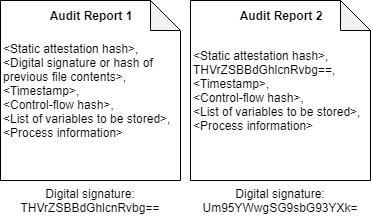
\includegraphics[scale=0.5]{Files.png}
  \caption{The contents of control-flow audit files}
  \label{fig:auditFiles}
\end{figure}

\section{Provisioning}

\subsection{Instrumentation}

The existing binary will be instrumented either prior to loading or during the loading (bootloading process). Instrumentation means replacing instructions from the compiled code with ones which are used for attestation.

\subsection{Initial attestation}

All software will be scrutinised with an initial attestation upon initial commissioning.

\subsection{Secure world}

Secure world applications need to be signed before they are loaded (reference some sort of ARM document).


\section{Chapter Summary}
Building a control-flow graph (CFG) has been an open problem in academia. There are a handful of software packages which aim to offer this functionality (usually as a bi-product of other functionality such as compilation or reverse engineering). The most promising solution, angr \cite{Shoshitaishvili2016}, showed promise, however it only produced single BBL (basic clock) to BBL edges, rather than complete paths. This could be symptomatic of using CFGs as a basis for control-flow integrity (CFI) protection, whereas perhaps generating a collection of all valid paths would provide a superior basis for ensuring secure execution. Based on evaluations taken place, `angr' framework would most likely be the tool used in the proposed solution.

To trace control-flow it is has been suggested that existing binaries should go through an instrumentation process, where instructions which trigger transitions between BBLs are replaced with code which jumps execution to a trampoline (provided by the solution). This trampoline then sends the control-flow information to an application existing in the ``secure world'' which records said information. Execution is then transferred back to the original destination.

Additional details can be added to attestation reports via an API provided by the solution. This additional information may be important variables (which the developer of the application may which to keep track of) or environmental information such as other processes running on the device. Allowing these additions represents an increase in functionality compared to standard attestation, as important information can be bound to a record of the prior control-flow.

\chapter{Security Analysis} \label{chapterSecurityAnalysis}
\section{Security Analysis}

The solution presented fits with the security requirements in the following ways:
\begin{enumerate}
	\item \textbf{Works with compiled binaries}: The solution works with compiled binaries, where the binaries go through an instrumentation process.
	\item \textbf{Works with external binaries}: As with compiled binaries, external binaries will have to undergo instrumentation.
	\item \textbf{Works with embedded systems}: ARM TrustZone has been implemented on Cortex M processors which are widely used in embedded systems. Key storage and external storage will need to be in place for an embedded system to make use of this solution.
	\item \textbf{Granularity}: The solution provides granularity down to a basic block (BBL) level.
\end{enumerate}

Obvious vulnerabilities in the solution are the breach of the `secure world' where the measurement engine is manipulated to create `good' attestation files, deletion of files and resulting loss of audit capabilities (a backup method would somewhat alleviate this problem) and cloning of audit files. Cloning of audit files represents a significant problem due to the fact that this is an offline process, so a method will need to be used to ensure freshness of files, for example a tamper-proof date-time stamp.

Granularity to an instruction level can only be provided by a hardware solution which intercepts each instruction.

\fi

\ifnotesincluded
\chapter{Conclusion} \label{chapterConclusion}
The objective of this project was to investigate secure software execution in embedded systems and apply this knowledge towards a proposed method of providing audit records of control-flow.

In order to achieve these objectives, it was first important to understand the principles of control-flow: how instructions within an application transition into one another, how we can model these transitions using control-flow graphs (CFG) and how if the instruction execution diverts away from following the CFG for a particular application this represents a violation of control-flow integrity (CFI), which is an important principal when considering secure software execution. Attacks on secure software execution were identified and examined as were the elements of execution flow which are vulnerable to manipulation. A literature review was carried out on the subject of secure software execution as well as software-hardware binding, as the two concepts converge in that they require close control\slash monitoring of software execution, and that by utilising dedicated cryptographic keys in ensuring secure software execution it is possible to leverage the mechanisms to provide software-hardware binding. Leading solutions providing static attestation and CFI attestation\slash protection were analysed and assessed against a set of defined requirements. Finally a proposed solution, with the goal of providing audit records of control-flow, was described.

The solution presented was defined after the introduction and literature review and inspired by the solutions identified in the comparison chapter. It was decided that the solution would be software-based and leverage the security features provided by TrustZone functionality of the ARMv8-M architecture to remove the requirement for additional hardware. The solution consists of several phases: performing analysis on the compiled binary to produce a CFG (for use as a comparison when audit records are referred to at a later point); undertaking an instrumentation phase where instructions within the binary are replaced with ones facilitating control-flow monitoring; provisioning the binary to the device; performing an initial static attestation report on the ``normal-world'' and ``secure-world'' memory; before sampling the control-flow history of the application and storing it along with important operating variables in signed and hash-chained files.

A security analysis of the proposed solution did find that a software-based method leveraging ARM TrustZone met several of the objectives set at the start of the project, and advanced existing CFI solutions in a manner which allows offline auditing. However, the analysis also found that a hardware-based solution would offer many more advantages, such as removing execution overhead from the primary processor and enabling monitoring at an individual instruction level of granularity. The analysis also found that the use of offline methods for monitoring control-flow were vulnerable to several attacks such as replay and proxy-based attacks, however this could be mitigated against through the combined use of tamper resistant real time clocks and digital signatures.

Further work could include implementing the proposed solution, testing the overhead introduced by the solution and implementing a similar solution using hardware (for example using an FPGA with a softcore processor).

We predict that control flow integrity will become part of the hardware offering for embedded systems in order to provide secure software execution. Much like how TPMs have grown in prominence over recent years, it important that secure software execution becomes a feature on offer to embedded system designers. Challenges will include the efficient generation of full-coverage CFGs, or indeed removing the requirement for their generation. Additionally, reducing the requirement for binary instrumentation or making it a seamless part of the provisioning process is a vital step to be made.


\fi

\begin{sloppypar}
\printbibliography
\end{sloppypar}
\end{document}